\chapter{Princip postačitelnosti, podmíněnosti, věrohodnosti, zastavovací pravidlo sekvenčního principu, vztahy.}
\begin{description}
	\item[SUFFICIENCY princip:] Máme experiment $\mathcal{E}$ závislý na~$\t$, pozorování $x,y$ a~nechť je v~$\mathcal{E}$ k~dispozici postačující statistika $T$ (PS). Víme-li, že $T(x)=T(y)$,~chceme, aby závěry o~$\t$ na~základě $x$ nebo $y$ byly shodné. ($T$ je PS pokud rozdělení $X|T(X)=t$ nezávisí na~$\t$).
	
	\item[LIKELIHOOD princip:] Informace o~$\t$ nesená $x$ je zcela obsažena ve~věrohodnostní funkci $f_\X(\textbf{x},\t)=L$. Navíc, pokud máme pozorování $x_1$ v experimentu $\mathcal{E}_1$ a~$x_2$ v~experimentu $\mathcal{E}_2$ taková, že 
	$$ L_1(\t|x_1)=c L_2(\t|x_2),\quad\forall\t\in\Theta,$$
	pak chceme, aby závěry o~parametru $\t$ v~obou experimentech byly shodné. Označíme to $\mathrm{Ev}(\mathcal{E}_1,x_1)=\mathrm{Ev}(\mathcal{E}_2,x_2)$ (Ev jako Evidence). 
	\item[CONDITIONALITY princip:] Nechť máme dostupné $\mathcal{E}_1,\mathcal{E}_2$. Definujeme $\mathcal{E}^*$ experiment tak, že vybereme náhodně mezi~$\mathcal{E}_1 \vee \mathcal{E}_2$, a~v~tom vybraném naměříme $x_j,~j=1\vee 2$. Chceme, aby $\Ev\big(\mathcal{E}^*,(j,x_j)\big)=\Ev(\mathcal{E}_j,x_j),~\forall j,\forall x_j$.
	\item[STOPPING rule:] Máme posloupnost experimentů $\mathcal{E}_1,\mathcal{E}_2,...$ a zastavovací pravidlo $\tau$, které zastavuje posloupnost v~bodě $\mathcal{E}_n$. Jsou naměřeny $\textbf{x}=\Big( x_1^{\mathcal{E}_1},x_2^{\mathcal{E}_2},...,x_n^{\mathcal{E}_n} \Big)$, ozn. $\{ \mathcal{E}_1,...,\mathcal{E}_n,\tau \}$ (sekvenční). Chceme, aby $\Ev\Big( \{ \mathcal{E}_1,...,\mathcal{E}_n,\tau \},\textbf{x} \Big)$ závisela na~$\tau$ pouze prostřednictvím $\textbf{x}$, tzn. $$\Ev\Big( \{ \mathcal{E}_1,...,\mathcal{E}_n,\tau_1 \},\textbf{x} \Big)=\Ev\Big( \{ \mathcal{E}_1,...,\mathcal{E}_n,\tau_2 \},\textbf{x} \Big),~\forall \textbf{x}.$$
	\item[BAYESOVSKÝ princip:] Taková procedura, která využívá k~rozhodnutí o~parametru $\t$ aposteriorní hustotu $\pi(\t,\textbf{x})=\frac{f_\X\cdot\pi(\t)}{\int f_\X\cdot\pi(\t) d\t}$, např. $\widehat{\t}_B=''\EE{\pi(\t,\textbf{x})}''=\E^\pi(\t|\textbf{x})$.
\end{description}

\begin{example}
	Mějme $\mathcal{E}_j..x_j\in\Ran(X_j)$, kde $X_j\sim f(x_j,\t),~\forall j\in 1,2,...$. Teoricky můžeme jít až do~nekonečna, ale někdy chceme experiment zastavit, abychom mohli vyhodnotit data. Definujeme tedy $\tau$ jako zastavení v~bodě $n$, pokud $\textbf{x}:=(x_1,...,x_n)\in\Ran(X_1)\times\Ran(X_2)\times...\times\Ran(X_n)\equal{ozn}\Aa_n$. Platí, že
	$$ L(\t|\textbf{x})\equal{id}\Big(\prod f_{X_j}(x_j,\t) \Big)\cdot I_{\Aa_n}(\textbf{x})\equal{non~id}f(x_1|\t)f(x_2|x_1,\t)...f(x_n|x_1,x_2,...,x_{n-1},\t)I_{\Aa_n}(\textbf{x}).$$
	Vidíme, že $L(\t|\textbf{x})$ nezávisí na zastavovacím pravidlu $\tau$ přímo, ale pouze prostřednictvím $\textbf{x}$. Tedy pokud platí $L$ princip, potom platí i $SR$ princip.
\end{example}
\begin{example}
	Máme TV seriál. Označme $\t\in[0,1]$ jako sledovanost daného dílu. Bylo zjištěno, že 9 diváků seriál sledují a~3 nikoliv (to jsou naše data). Problém je, že nevíme, jakým způsobem byla data naměřena. 
	\begin{description}
		\item[$\mathcal{E}_\mathrm{I}:$] vybráno $n=12$ lidí, otestováno, získána data (9DIV,3NEDIV). Máme tedy náhodnou veličinu $X$ jako počet diváků z~$n=12$ nezávislých opakování. Z~toho plyne, že $X\sim \Bi(12,\t)$. Máme napozorováno $X(\omega)=x=9$.
		\item[$\mathcal{E}_\mathrm{II}:$] vybíráme $x$ osob a~testujeme tak dlouho, dokud nezískáme $3$ nediváky. Při~tomto způsobu ale měření probíhá zcela odlišně. Tedy celkový počet otestovaných osob \mbox{$N\sim\mathrm{NegBi}(3,1-\t)$}. Napozorováno tedy bylo $N(\omega)=n=12$.
	\end{description}
	$$ \text{Vidíme, že}\qquad L_\mathrm{I}(\t,\mathcal{E}_\mathrm{I})=c_1\t^9(1-\t)^3\quad\propto\quad L_\mathrm{II}(\t,\mathcal{E}_\mathrm{II})=c_2\t^9(1-\t)^3,\quad \forall\t\in[0,1]. $$
	Pokud platí LIKELIHOOD princip, pak $\Ev\big(\mathcal{E}_\mathrm{I},(9)\big)=\Ev\big(\mathcal{E}_\mathrm{II},(12)\big)$ (takže vlastně na~zastavovacím principu nezáleželo).
\end{example}

\begin{example}
	Máme laboratoř a~v~ní dva přístroje:
	\begin{itemize}
		\item 1. přístroj přesný $X_1\sim\NN(\t,0.1)$ [$\mathcal{E}_1$] (vytížený),
		\item 2. přístroj nepřesný $X_2\sim\NN(\t,10)$ [$\mathcal{E}_2$] (volný).
	\end{itemize}
	Rozhodování o~$\t$: 95\%-interval spolehlivosti pro~$\t$.\begin{enumerate}[A)]
		\item osobně, naměříme $x_1$ v $\mathcal{E}$, pak spočteme délku ($IS_{95\%}$)$=0.62$ (na 2. přístroji nezáviselo).
		\item vyšleme laborantku. která nese data (ale neví, ze~kterého přístroje jsou, prostě mohla použít i~volný přístroj). Máme model $\Phi=\beta\NN(\t,0.1)+(1-\beta)\NN(\t,10)$, kde $\beta$ vyjadřuje míru obsazenosti 1. přístroje. Pak zjistíme $x$ jako délku($IS_{95\%}$) s~hodnotou $5.19$.
	\end{enumerate}
\end{example}
\begin{theorem}
	$S\wedge C\Leftrightarrow L\Rightarrow SR$. Implikace $L\Rightarrow C$ a $L\Rightarrow S$ jsou důležité, protože $B~''\Rightarrow'' L$.
	\begin{proof}
		\begin{enumerate}[$B"\Rightarrow"L$:]
			\item Mějme $\mathcal{E}_1,\mathcal{E}_2$, $x_1,x_2$ a~předpokládejme, že $L_1(\t)=c L_2(\t)$. Ptáme se, jestli je $\Ev(\mathcal{E}_1,x_1)=\Ev(\mathcal{E}_2,x_2)$. Víme, že $$ \underbrace{\pi_1(\t|x_1)}_{\sim\mathcal{E}_1}=\frac{f_{X_1}(x_1|\t)\pi(\t)}{\int f_{X_1}(x_1|\t)\pi(\t)\d\t}=\frac{c f_{X_2}\pi}{\int c f_{X_2}\pi\d\t}=\underbrace{\pi_2(\t| x_2)}_{\sim\mathcal{E}_2}.$$
		\end{enumerate}
	\begin{enumerate}[$L\Rightarrow S$:]
		\item Nechť T je PS pro exponenciální $\mathcal{E}$ a~nechť máme data $x_1^0,x_2^0$ (nula značí konkrétní výběr, nikoliv obecný), taková, že $T(x_1^0)=T(x_2^0)$. Máme k~dispozici Neymannův faktorizační teorém, $X\sim f(x,\t)$, pak $T(X)$ je PS právě tehdy, když $f(x|\t)=h(x)g\big(T(x),\t \big),~\forall\t$. Potom tedy 
		$$ L(\t|x_1^0)=f(x_1^0,\t)=h(x_1^0)g\big( T(x_1^0),\t \big)=\frac{h(x_1^0)}{h(x_2^0)}\underbrace{h(x_2^0)g\big(T(x_2^0),\t \big)}_{f(x_2^0,\t)=L(\t|x_2^0)},\quad\forall\t.$$
		Z toho vyplývá (dle L principu), že $\Ev(\mathcal{E},x_1^0)=\Ev(\mathcal{E},x_2^0)$.
\end{enumerate}
\begin{enumerate}[$L\Rightarrow C$:]
	\item Uvažujeme experiment $\mathcal{E}^*$ tak, že $(\mathrm{I},X_\mathrm{I})=X^*$, $I=1\vee 2,~X_I=x_1\vee x_2$. 
	Dále potom \[
	\begin{split}
	L^*\big(\t|(j,x_j)\big)&=\PP\big(X^*=(j,x_j) \big)=\PP(I=j\wedge X_{I=j}=x_j)=\PP(I=j)\PP(X_j=x_j)=\\&=0.5f(x_j,\t)=0.5 L_j(\t,x_j)
	\end{split}
	\]
	pro $\forall\t,~\forall x_j$, tzn. $L^*=c L_j$. Potom tedy dle Likelihood principu máme $$\Ev\big(\mathcal{E}^*,(j,x_j) \big)=\Ev\big(\mathcal{E}_j,x_j \big),~\forall j,~\forall x_j.$$
\end{enumerate}
	\end{proof}
\end{theorem}

\section{Statistical decision theory}

\begin{define}
	Označíme $\Dd$ jako množinu možných rozhodnutí o~$\t$, případně $\tau(\t)$. Dále potom $\delta\in\Dd$. $L:\Theta\times\Dd\to[0,+\infty)$ nazýváme \textbf{loss function} (ztrátová funkce) a~$L(\t,\delta)$ je \textbf{míra ztráty} (shody, neshody), pokud pro~$\t$ použijeme rozhodnutí $\delta$.
	
	Označme dále $\Rr$ jako \textbf{reward space}, který je spojen s~$\Dd$, tj. $\forall\delta\in\Dd$ přiřazujeme $r\in\Rr$ ($\delta\leftrightarrow r$). Předpokládejme dále, že na~$\Rr$ existuje úplné uspořádání ($\leq$) tak, že \begin{enumerate}[{A}1)]
		\item $\forall r_1,r_2\in\Rr,~r_1\leq r_2 \vee r_2\leq r_1$,
		\item $\forall r_1,r_2,r_3\in\Rr,~r_1\leq r_2 \wedge r_2\leq r_3~\Rightarrow~r_1\leq r_3$. 
	\end{enumerate}Z~toho vyplývá, že nastává právě jedna varianta
$$ r_1<r_2,\quad r_2<r_1,\quad r_1=r_2~(r_1\sim r_2).$$
Poslední rovnost není myšlena jako číselná rovnost, ale spíše jako ekvivalence (peníze pro~nás můžou mít stejnou cenu, jako získané znalosti).

	Nad $\Rr$ definujeme prostor $\mathcal{P}$ pravděpodobnostních distribucí náhodné veličiny $r$ ($r\sim\PP\in\mathcal{P}$). Předpokládejme, že na~$\mathcal{P}$ existuje úplné uspořádání ($\leq$) analogické s A1) a A2).
\end{define}

Motivace: označme $d_i$ jako investice do~$i$-té společnosti. Na~konci roku pak očekáváme dividendy $r_i$. $(d_i)_1^k...(r_i)_1^k$ a celková dividenda $r=\sumin r_i$ má pak rozdělení $\PP=\PP_1\ast...\ast\PP_k$, které lze aproximovat z CLT.

\begin{define}
	Funkci $U$ na~$\Rr$ nazveme \textbf{užitkovou} (utility function), pokud $\forall P,Q\in\mathcal{P}$ platí, že 
	$$ P\leq Q\quad\Leftrightarrow\quad\E^P\big[U(r)\big]\leq\E^Q\big[U(r)\big],$$ kde $r$ je náhodná veličina. Pokut to jde, můžeme například volit $U(r)=r$.
\end{define}
\begin{remark}
	Pokud má $\mathcal{P}$ vhodné vlastnosti, pak existuje užitková funkce $U(r)$, která zachovává dané uspořádání $\mathcal{P}$ a pro~ztrátu $L(\t,\delta)\geq 0$ můžeme volit $L(\t,\delta)=U(\t,\delta)=-\E[U(r)]+c$, kde konstantu $c$ přičítáme proto, abychom se~nedostali do~záporných čísel. Tím zajistíme, že pokud budeme provádět minimalizaci $L$, pak provádíme i~maximalizaci užitku.
\end{remark}
\begin{example}[volba L]
		Předpověď počasí v~Kanadě. Předpovědi jsou ve~tvaru "pravděpodobnost, že zítra bude pršet je $p$". Předpovědi od~různých společností chceme nějak porovnat. Sledujeme tedy 365 dní všechny předpovědi a~přiřadíme každému předpovídateli jeho použitá $p_1,...,p_N$. Definujeme relativní četnost $$\t_j=\frac{\text{\# dnů, kdy pršelo a~byla použita }p_j}{\text{\# dnů, kdy byla použita }p_j},\quad j\in\widehat{N}.$$ Sestavíme ztrátovou funkci (použil De Groot v~roce 1988) $$L(\boldsymbol{\t},\textbf{p})=\sum_{j=1}^N q_j(p_j-\t_j)^2+\sum_{i=1}^N q_i\ln q_i,$$ kde $q_j=\frac{\text{\# použití }p_j}{365}$ a~$H(\textbf{q})=-\sum_1^N q_j\ln q_j\geq 0$ je entropie rozdělení $\{q_j\}_{j=1}^N$. Suma $\sum_{i=1}^N q_i\ln q_i$ pak penalizuje předpovědi, které jsou nevyvážené, protože pro systém neuspořádanosti (rovnoměrné rozdělení $q_j=\frac{1}{N},~\forall j$) je $H(\textbf{q})$ maximální.
		
		Člen $\sumjn q_j(p_j-\t_j)^2$ nemusí být nutně na~druhou, můžeme brát závorku i~v~absolutní hodnotě, případně ji umocnit na~$\alpha\in(0,2)$ a regulovat tak robustnost $L(\t,p)$. Tím vším vstupuje do~našeho problému tzv. \textbf{Apriorno}, musíme totiž dopředu vědět některé informace, třeba $X\sim f(x,\t)$, tvar $L(\t,\delta)$. 
\end{example}

\section{Rozhodovací principy statistiky}

\begin{define}
	Mějme $\Theta$, $\mathcal{F}=\big\{ f(x,\t):\t\in\Theta \big\}$,~$\mathscr{D}$, kde $\delta\in\mathscr{D}$ a~$\chi$ jako výběrový prostor pro~data $\textbf{x}$. Funkci $\delta:\chi\to\mathscr{D}$ nazýváme \textbf{rozhodovací funkce}, $\delta(\textbf{x})=\delta\in\mathscr{D}$. 
\end{define}
\begin{description}
	\item[Metoda A) minimalizace L:] $\delta_L(\textbf{x})=\argmin\limits_{\delta\in\mathscr{D}} L\big(\t,\delta(\textbf{x})\big),~\forall \t\in\Theta,~\forall\textbf{x}\in\chi$. Avšak je obtížné, až nemožné, takto obecně stejnoměrně minimalizovat.
	\item[Metoda B) Riziková funkce] (risk function) je funkce $\RF:\Theta\times\mathscr{D}\to\R^+$, definovaná jako $$\RF(\t,\delta)=\E_\t L\big(\t,\delta(\textbf{X})\big)=\int L\big(\t,\delta(\textbf{x})\big)f_\textbf{X}(\textbf{x},\t)\d\textbf{x}.$$
	Rizikovou funkci také nazýváme jako \textit{střední ztrátu}. Definujeme $\delta_U=\argmin\limits_{\delta\in\mathscr{D}} \RF(\t,\delta),~\forall\t\in\Theta$.
	
	\begin{figure}[h]
		\centering
		\begin{tikzpicture}
		\node[inner sep=0pt] (pic) at (0,0)
		{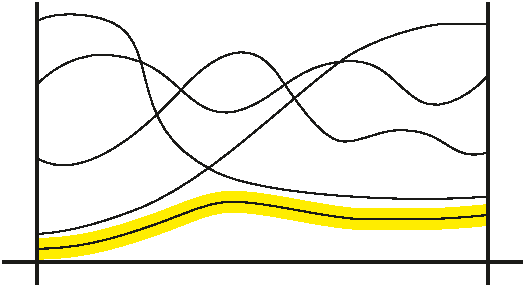
\includegraphics[width=7.5cm]{pictures/picture_3_2.pdf}};
		\draw [color=black](3.4,2.0) node[anchor=north west] {$ \text{R}(\theta, \delta_1 )
			$};
		\draw [color=black](3.4,1.3) node[anchor=north west] {$ \text{R}(\theta, \delta_2 )
			$};
		\draw [color=black](3.4,0.2) node[anchor=north west] {$ \text{R}(\theta, \delta_3 )
		$};
	\draw [color=black](3.4,-0.4) node[anchor=north west] {$ \text{R}(\theta, \delta_4 )
	$};
\draw [color=black](3.4,-.8) node[anchor=north west] {$ \text{R}(\theta, \delta_5 )
$};
		\end{tikzpicture}
		\caption{HPD Region.}
	\end{figure}
	
	Ne vždy lze najít stejnoměrně nejlepší řešení. V~takovém případě pak přejdeme na~prostor $\mathscr{D}_0\subset\mathscr{D}$, kde již lze najít stejnoměrně nejlepší řešení (typicky vypustíme některé rizikové funkce). Můžeme tedy optimalizovat na různých prostorech rozhodovacích fukncí, např.
	\begin{enumerate}[a)]
		\item  Prostor rozhodovacích funkcí, které jsou nestranné -- pak vede na~UMVUE.
		\item $\mathscr{D}_0$ takový, který je prostorem ekvivariantních rozhodovacích funkcí na modelech invariantních na~určitou transformaci (např. posunutí, přeškálování, tzn. tzv. \textbf{lokálně-měřítkové modely}).
	\end{enumerate}
	
	Problémy této stejnoměrně optimální strategie: \begin{enumerate}[a)]
		\item $\delta_1,\delta_2$ a~k~nim $\RF(\t,\delta_1),\RF(\t,\delta_2)$ takové, že se~kříží -- nejsme schopni rozhodnout, která strategie je lepší.
		\item Minimalizujeme $\E L$, ale předpis $\delta$ (odhadce) nezávisí na~$\textbf{x}$ - výběr nejlepšího $\delta$ nezávisí na~naměřených datech.
		\item Na~rozmyšlenou je následující příklad \ref{example:problemy}.
	\end{enumerate}
\end{description}

\begin{example} \label{example:problemy}
	Mějme $X=\begin{cases}
	\t-1 & \text{s pravd. } \frac{1}{2}, \\ \t+1 & \text{s pravd. } \frac{1}{2},
	\end{cases}~\t\in\R,~\mathscr{D}=\R$. Volme
	$ L(\t,\delta)=1-I_\t(\delta)$, kterou nazýváme "0-1" ztrátovou funkci.
	
	\begin{enumerate}[1)]
		\item Máme $(x_1,x_2)$ data a~sestrojíme $\delta_0=\frac{x_1+x_2}{2}=\begin{cases}
		\t\\\t-1\\\t+1
		\end{cases}$ symetricky kolem~$\t$. Potom
		$$ \RF(\t,\delta_0)=\E L(\t,\delta_0)=1-\E I_\t(\delta_0)=1-\PP(\delta_0=\t)=1-\PP(X_1\neq X_2)=\frac{1}{2}.$$ To nám říká, že střední ztráta je rovna $\frac{1}{2}$, tzn. že v~průměru 50\% případů bude příznivých (trefíme se~do~parametru).
		\item Máme data $(x_1,x_2)$ a~sestrojíme $\delta_1=x_1+1=\begin{cases}
		\t\\\t+2
		\end{cases}$ nesymetricky rozdělené kolem~$\t$. Potom
		$$\RF(\t,\delta_1)=...=1-\PP(\delta_1=\t)=1-\PP(X_1=\t-1)=\frac{1}{2}.$$
	\end{enumerate}
	Srovnání $\delta_0$ a~$\delta_1$ nelze rozhodnout na~základě $\RF$-strategie. 
\end{example}

\chapter{Nezkontrolováno}
\begin{description}
	\item[Metoda c) Strategie MINIMAXní] $\sup\limits_{\t\in\Theta} \RF(\t,\delta)$ nazýváme ''\textit{maxní}''(\textit{supremální}) riziková funkce a~je rovna $\RF_{\sup}(\t,\delta)$. Definujeme 
	$$ \delta_0=\argmin\limits_{\delta\in\mathscr{D}}\RF_{\sup}(\t,\delta)=\argmin\limits_{\delta\in\mathscr{D}}\underbrace{\sup\limits_{\t\in\Theta}\underbrace{\E_\t L(\t,\delta(\X))}_{\RF(\t,\delta)}}_{r_{\sup}\in\R_0^+}.$$
\end{description}

\begin{define}
	Definujeme \textbf{minimaxní riziko} ve~tvaru $\overline{\RF}=\inf\limits_\delta\sup\limits_\t\RF(\t,\delta)$.
\end{define}

\begin{figure}[h]
	\centering
	\begin{tikzpicture}
	\node[inner sep=0pt] (pic) at (0,0)
	{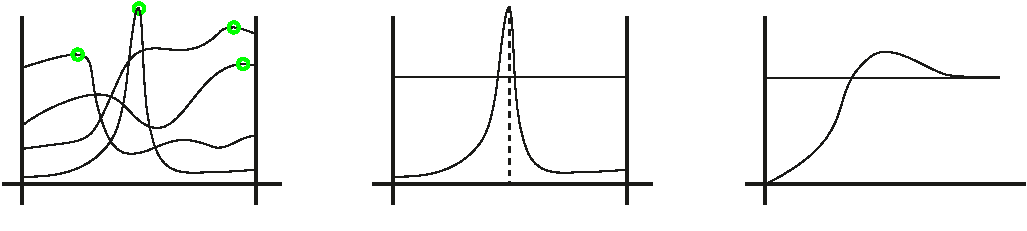
\includegraphics[width=15.0cm]{pictures/picture_3_4.pdf}};
	\draw [color=black](3,0.5) node[anchor=north west] {$ \delta $};
	\draw [color=black](0,-0.3) node[anchor=north west] {$ \theta $};
	\end{tikzpicture}
	\caption{1: zeleně suprema, nejmenší supremum je delta3 2: lepší je delta2, protože ač je riziko vysoké, jeho šance je velice malá - toto je nevýhoda minimaxní strategie 3: delta2 jen lehce překmitne delta1 a~pak se~k~němu blíží asymptoticky}
\end{figure}

\begin{remark}
	Analogie z~teorie her. Pokud máme 2 hráče, kteří mají antagonický vztah (snaží se~navzájem poškodit a~nezáleží jim na~ztrátě). První hráč udělá nějaký tah. Druhý hráč pak udělá tah, který co nejvíc poškodí 1. hráče. První hráč to předvídá a~snaží se~tedy minimalizovat nejhorší možnou ztrátu.
\end{remark}

\begin{remark}
	Stavba naftové plošina v~Severním moři. Máme vstupy=parametry (teplota, vítr, příliv, bouřky, lidský faktor,...) a~rozhodujeme se, jak plošinu postavit.
	\begin{figure}[h]
		\centering
		\begin{tikzpicture}[line cap=round,line join=round,>=triangle 45,x=1.5cm,y=1.5cm]
		\clip(-1.25,-0.27) rectangle (7,3.03);
		\draw [->] (0,-0.48) -- (0,3);
		\draw [->] (-0.25,0) -- (5,0);
		\draw [dash pattern=on 2pt off 2pt] (4.27,-0.38)-- (4.27,2.55);
		\draw [dash pattern=on 2pt off 2pt] (-0.25,2.55)-- (4.27,2.55);
		\draw [shift={(0.04,2.55)}] plot[domain=-1.595:0,variable=\t]({1*0.63*cos(\t r)+0*0.63*sin(\t r)},{0*0.63*cos(\t r)+1*0.63*sin(\t r)});
		\draw [shift={(0.02,0)}] plot[domain=0:1.595,variable=\t]({1*0.74*cos(\t r)+0*0.74*sin(\t r)},{0*0.74*cos(\t r)+1*0.74*sin(\t r)});
		\begin{scriptsize}
		\draw [color=black] (1.64,1.4)-- ++(-1.5pt,-1.5pt) -- ++(3.0pt,3.0pt) ++(-3.0pt,0) -- ++(3.0pt,-3.0pt);
		\draw [color=black] (0.88,1.52)-- ++(-1.5pt,-1.5pt) -- ++(3.0pt,3.0pt) ++(-3.0pt,0) -- ++(3.0pt,-3.0pt);
		\draw [color=black] (1.98,1.9)-- ++(-1.5pt,-1.5pt) -- ++(3.0pt,3.0pt) ++(-3.0pt,0) -- ++(3.0pt,-3.0pt);
		\draw [color=black] (0.4,0.34)-- ++(-1.5pt,-1.5pt) -- ++(3.0pt,3.0pt) ++(-3.0pt,0) -- ++(3.0pt,-3.0pt);
		\draw [color=black] (3.2,1.8)-- ++(-1.5pt,-1.5pt) -- ++(3.0pt,3.0pt) ++(-3.0pt,0) -- ++(3.0pt,-3.0pt);
		\draw [color=black] (3.14,0.96)-- ++(-1.5pt,-1.5pt) -- ++(3.0pt,3.0pt) ++(-3.0pt,0) -- ++(3.0pt,-3.0pt);
		\draw [color=black] (1.98,0.52)-- ++(-1.5pt,-1.5pt) -- ++(3.0pt,3.0pt) ++(-3.0pt,0) -- ++(3.0pt,-3.0pt);
		\draw [color=black] (0.98,1.96)-- ++(-1.5pt,-1.5pt) -- ++(3.0pt,3.0pt) ++(-3.0pt,0) -- ++(3.0pt,-3.0pt);
		\end{scriptsize}
		\draw [color=black](-0.6,2.3) node[anchor=north west] {$ v_{\text{max}}$};
		\draw [color=black](-0.6,3) node[anchor=north west] {vítr};
		\draw [color=black](0,0) node[anchor=north west] {$ t_\text{min} $};
		\draw [color=black](3.3,0) node[anchor=north west] {$ +50^\circ C $};
		\draw [color=black](5,0.2) node[anchor=north west] {teplota};
		\draw [color=black](-0.4,0.4) node[anchor=north west] {$ 0 $};
		\end{tikzpicture}
		\caption{}
		\label{fig:p51}
	\end{figure}
	
\end{remark}
\begin{description}
	\item[Metoda d) Bayesovská riziková funkce] $r(\pi,\delta):\Pi=\{ \pi\text{ apriorní rozdělení pro~}\t \}\times\mathscr{D}\to\R_0^+$.
	$$ r(\pi,\delta)=\E^\pi\big[ R(\t,\delta) \big]=\int\limits_{\Theta}R(\t,\delta)\pi(\t)\d\t=\int\limits_{\Theta}\Big( \int\limits_{\chi}L\big(\t,\delta(\textbf{X})\big)f_\textbf{X}\d\textbf{x} \Big)\pi(\t)\d\t.$$
	Definujeme $\delta^\pi=\argmin\limits_{\delta\in\mathscr{D}}r(\pi,\delta)$, za~předpokladu existence, jako \textbf{Bayesovskou rozhodovací funkci}. Číslo $r(\pi)=r(\pi,\delta^\pi)$ nazýváme \textbf{Bayesovské (apriorní) riziko}.  
\end{description}
\begin{remark}
	Mějme $\pi$ fixní, $\delta_1\leq\delta_2~\Leftrightarrow~r(\pi,\delta_1)\leq r(\pi,\delta_2)$ uspořádané v~$\R^1$. Rozšíření i~na~\textbf{nevlastní apriorní hustoty} (inf.), pokud $r(\pi)<+\infty$. ($r_\text{inf}(\pi)=\inf_\delta r(\pi,\delta)<+\infty$)
\end{remark}
\begin{example}
	Mějme $X\sim\underbrace{\NN(\t,1)}_{f_X}$, $\t\in\R,~\pi(\t)=1$ (konstantní) na~$\R$ (nevlastní hustota). Pak
	$$ \pi(\t|x)=\frac{f_X \pi(\t)}{\int_{-\infty}^{+\infty}f_X \pi(\t)\d\t}=\frac{1}{c}\e{-\frac{1}{2}(\t-x)^2}=\frac{1}{\sqrt{2\pi}}\e{-\frac{1}{2}(\t-x)^2}.$$
	\[\begin{split}
	\delta^\pi(\textbf{x})&=\EE{\pi(\t|x)}=\E\NN(x,1)=x\text{ obecněji }\overline{x}_n\\
	r(\pi)&= r(\pi,\delta^\pi)=\E^\pi R=\E^\pi[\E^f L_2]\equal{def}\E^\pi\big[ \E^f\underbrace{\big(\t-\delta^\pi(X) \big)^2}_{L_2} \big]=\E^\pi\E^f(\t-X)^2=\\&=\E^\pi\big[ \E^f(X-\E^fX)^2 \big]=\E^\pi(\sigma^2)=\int_{-\infty}^{+\infty}\sigma^2\cdot 1\d\t=+\infty
	\end{split}
	\]
\end{example}
\begin{define}
	Máme $L,~f_{\X},~\pi(\t)$. Definujeme \textbf{aposteriorní Bayesovskou rizikovou funkci} vztahem
	$$ \rho(\pi,\delta(\textbf{x})|\textbf{x})=\E^\pi\big[ L\big(\t,\delta(\textbf{x})\big)|\textbf{x} \big]=\int L\big(\t,\delta(\textbf{x})\big)\pi(\t|\textbf{x})\d\t.$$ 
\end{define}

\begin{description}
	\item[Metoda e) ???] definujeme $\delta_\rho^\pi(\textbf{x})=\argmin\limits_{\delta(\textbf{x})}\rho(\pi,\delta(\textbf{x})|\textbf{x})$ za~předpokladu existence pro~skoro všechna $\textbf{x}$.
\end{description}

\begin{remark}
	Výhoda této definice je, že $\delta_\rho^\pi$ závisí přímo na~datech $\textbf{x}$. Nevýhoda pak je, že musíme minimalizaci dělat opakovaně pro~každá data $\textbf{x}$.
\end{remark}
\begin{theorem}
	Máme-li $\delta_\rho^\pi$ pro s.v. $\textbf{x}$, pak $\delta_\rho^\pi=\delta^\pi$, tj. je rovna s.v. Bayesovské rizikové funkci (D strategie $\delta^\pi=\argmin_\delta r(\pi,\delta)$).
	\begin{proof}
		\[
		\begin{split}
		\rho\big(\pi,\delta_\rho^\pi(\textbf{x})|\textbf{x}\big)&\leq \rho(\pi,\delta(\textbf{x})|\textbf{x}) \hspace{0.2cm} \text{pro s.v. } \textbf{x} \\
		\E^m\rho\big(\pi,\delta_\rho^\pi(\textbf{x})|\textbf{x}\big)&\leq \E^m\rho(\pi,\delta(\textbf{x})|\textbf{x})\text{, kde } m(\textbf{x})=\int_{\Theta}f(\textbf{x}|\t)\cdot \pi(\t)\d\t
		\end{split}
		\]
		kde
		\[
		\begin{split}
		\E^m\rho(\pi,\delta(\textbf{x})|\textbf{x})&=\int\limits_{\chi}\Big( \int\limits_{\Theta} L(\t,\delta)\underbrace{\pi(\t|\textbf{x})}_{\frac{f\pi(\t)}{\int f\pi(\t)\d\t}=\frac{f\pi(\t)}{m(\textbf{x})}}\d\t\Big)m(\textbf{x})\d\textbf{x}\equal{Fubini}\int\limits_{\Theta}\Big( \underbrace{\int\limits_{\chi} L\big(\t,\delta(\textbf{x})\big)f(\textbf{x}|\t)\d\textbf{x}}_{\E^f L=R(\t,\delta)} \Big)\pi(\t)\d\t=\\&=\E^\pi\E^f L=r(\pi,\delta) \\
		\E^m\rho(\pi,\delta_\rho^\pi(\textbf{x})|\textbf{x})&=\{\text{Analogický postup}\}=r(\pi,\delta_\rho^\pi).
		\end{split}
		\]
		A tedy 
		$$ r(\pi,\delta_\rho^\pi)\leq r(\pi,\delta),~\forall\delta\quad \Rightarrow\quad \delta_\rho^\pi=\delta^\pi.$$
		Závěr: D strategie Bayes($\delta^\pi$) je rovna E strategii Bayes ($\delta_\rho^\pi(\textbf{x})$ pro s.v. $\textbf{x}$).
	\end{proof} 
\end{theorem}
Rozšíření: máme-li $\delta_\rho^\pi(\textbf{x})$ pro s.v. $\textbf{x}$ a~stane se, že $r(\pi)=+\infty$. Toto řešení $\delta^{\phi}$ nazveme \textbf{Zobecněnou Bayesovskou rozhodovací funkcí}.

Další výhody: $\pi(\t)$ a~máme data $\textbf{X}\sim f(\textbf{x},\t)\stackrel{\text{ÚBM}}{\longrightarrow}\pi(\t,\textbf{x})$ (ÚBM = úplný Bayes. model) update ($\widehat{\t}_B$ int. spol.). $\tilde{\pi}(\t)=\pi(\t|\textbf{x})$ nová data $\tilde{\textbf{X}}\sim\tilde{f}(\tilde{\textbf{x}}|\t)\stackrel{\text{ÚBM}}{\longrightarrow}\tilde{\pi}(\t|\tilde{\textbf{x}})$ update ($\widehat{\t}_B^{\sim}$) apod. 

\begin{example}
	Varianta: lékař sleduje chorobu pacienta. 1. den $x_1\sim f(x|\t)$, kde $\pi_1(\t)$ je apriorní informace. Z~toho pak $\pi(\t|x_1)$. 2. den naměří $x_2\sim f(x|\t)$. Z~toho pak $\pi_2(\t)=\alpha\pi(\t| x_1)+(1-\alpha)\tilde{\pi}_2(\t)\to \pi(\t|x_2,x_1)$. Pak n-tý den naměří $x_n$ a~proces se~opakuje.
\end{example}
\subsection*{Úloha predikce}
\begin{description}
	\item[KLAS. STAT.] Máme $X\sim f(x,\t)$, data $D\sim\textbf{x}=(x_1,...,x_n)$, realizaci $\textbf{X}=(X_1,...,X_n)$ a~hledáme predikci $X_{n+1}$. Pokud použijeme IID model, pak $X_{n+1}\sim f(x|\t)$ a~odhad $\widehat{\t}=\widehat{\t}(\textbf{x})=\widehat{\t}_{\mathrm{ML}}$. Z~toho pak $\widehat{f}_{ML}(x)=f(x,\widehat{\t}_\mathrm{ML})$ a~z~toho $X_{n+1}\sim\widehat{f}$.
	\item[BAYES. STAT.] \begin{enumerate}[a)]
		\item Máme $X\sim f(x|\t)$, data $D:\textbf{x}$ a~$\pi(\t)$ apriorní informaci. Z~toho získáme $\pi(\t|\textbf{x})$ a~z~toho $\widehat{\t}_B=\EE{\pi(\t|\textbf{x})}$. Z~toho už $\widehat{f}(x)=f(x|\widehat{\t}_B)$ a~potom $X_{n+1}\sim\widehat{f}$.
		\item $\tau(\t)=f(x|\t)$, $\pi(\t)$, $\widehat{f}_B(x)=\widehat{\tau_B(\t)}$... $X_{n+1}\sim\widehat{f}_B$.
		\item \begin{define} Máme ÚBM pro $\X\sim f_{\X}(\textbf{x}|\t)$, $\pi(\t)$, $\pi(\t|\textbf{x})$. Pak definujeme \textbf{Bayesovskou prediktivní hustotu} $f_B^{PR} $ vztahem
		$$ f_B^{PR}(t|\textbf{x}\sim\text{data})=\int\limits_{\Theta} \underbrace{f_X(t|\t)\pi(\t,\textbf{x})}_{\phi(t,\t|\textbf{x})}\d\t=\EE{f_X(t|\t)|\textbf{x}}.$$
		\end{define}
		Potom
		$$ X_{n+1}\sim f_B^{PR}(x_{n+1}|\textbf{x}\text{ data})\quad\to\quad \PP(X_{n+1}>b)=\int\limits_b^{+\infty}f_B^{PR}\d x_{n+1}.$$
		Výhodou c) je potom to, že obsahuje ''plnou'' (ve smyslu integrálu) informaci ve~tvaru $\pi(\t|\textbf{x})$.
	\end{enumerate}
\end{description}
\begin{define}
	Mějme $P,Q\in\mathcal{P}$ a~definujeme \textbf{totální variaci} $\TV(P,Q)=\left\|P-Q\right\|_\TV=\sup\limits_{|g|\leq 1}\left| \int g(\X)\d P-\int g(\Y)\d Q \right|\equal{ASR}=\left|\begin{array}{l}
	p\equal{ozn}\frac{\d P}{\d \mu}\quad P,Q\ll\mu\\ q=\frac{\d Q}{\d \mu}
	\end{array}
	\right|=\int |p-q|\d\mu=\left\|p-q\right\|_{L_1}$.
\end{define}
\begin{define}
	Mějme posloupnost měr $(P_n)_1^{+\infty}$ a limitní míru $Q$. Řekneme, že $P_n$ konverguje silně ke $Q$, značíme $P_n\stackrel{\text{s}}{\rightarrow}Q$, pokud $\TV(P_n,Q)\to0$.
\end{define}
\begin{remark}{Slabá konvergence:}
	$$ P_n\wto Q~\Leftrightarrow~\int g(\X)\d P_n\to\int g(\Y)\d Q,\qquad \forall g\in C_B^{(0)}\text{ spojité a~omezené.}$$
\end{remark}
\begin{theorem}
	Nechť $P_n\stackrel{s}{\to}Q\Rightarrow P_n\wto Q$ (AN).
\end{theorem}
\begin{proof}
	 Nechť funkce $g$ je spojitá a~omezená, $|g|\leq M$. $g^\ast =g|_M$, $|g^\ast|\leq 1$. Pak
	$$ \left| \int g(\X)\d P_n-\int g(\Y)\d Q \right|=M\left| \int g^\ast(\X)\d P_n-\int g^\ast(\Y)\d Q \right|\leq M\cdot \left\| P-Q\right\|_\TV \stackrel{\text{LDCT}}{\longrightarrow} 0.$$
\end{proof}
\begin{theorem}[Scheffé theorem]
	Mějme $P_n,Q$ s~ASR$_\mu$, $p_n=\frac{\d P_n}{\d \mu}$, $q=\frac{\d Q}{\d \mu}$. Nechť dále hustota pravděpodobnosti $p_n\to q$ s.v. $\mu$. Pak $P_n\stackrel{s,(\TV)}{\longrightarrow}Q$. 
	\begin{proof}
		$$ \left| \int_A (p_n-q)\d\mu \right|\leq \int_A|p_n-q|\d\mu\leq \int_\R|p_n-q|\d\mu=2\int(p_n-q)^+\d\mu\to0,$$
		kde poslední rovnost platí, protože $\int(p_n-q)\d\mu=0$, a~tedy $\int(p_n-q)^+\d\mu-\int(p_n-q)^-\d\mu=0$.	\end{proof}
\end{theorem}
\begin{remark}
	Opakování. Z~01MAS víme, že pro~$\fregmle$ platí, že \begin{enumerate}[1)]
		\item $\supp f$ nezávisí na~$\t$,
		\item $f\in\mathcal{C}^{(3)}$ vzhledem k~$\t$ pro s.v. $x\in\supp f$,
		\item $\int f_\t'=0$ a~$\int f_{\t\t}''=0$,
		\item $\left( \mathbb{J}(\t)_{(\text{FIM})} \right)_{i,j}=\EE{\frac{\partial\log f}{\partial \t_i}\cdot\frac{\partial\log f}{\partial \t_j}}=-\EE{\frac{\partial^2 \log f}{\partial\t_i \partial \t_j}}$, $\mathbb{J}(\t)$ je PD a~konečná pro~$\forall\t\in\Theta$,
		\item $\forall\t_0~\exists H_{\t_0}~\exists M(\X)\in\LL_1(P_{\t_0})$ tak, že $\left\| \frac{\partial^3\log }{\partial \t^3}\right\|\leq M(x)$ na~$H_{\t_0}$, kde $\E_{\t_0}[M(X)]<+\infty$.
	\end{enumerate}
\end{remark}
\begin{theorem}[Bernstein - von Mises]
	Předpokládejme ÚBM: $X\sim f(x|\t)$ vzhledem k míře $\lambda$, která je $\sigma-$finitní, $\mathcal{F}=\left\{ f(x|\t):\t\in\Theta\subset \R^k \right\}$, $\Theta$ otevřená, $\t\sim\pi(\t)$ vlastní hustota, spojitá a $\pi(\t)>0$ (Tedy máme $\varphi(x,\t)=f\cdot\pi$, $m(\textbf{x})=\int f\cdot \pi\d\t$, $\pi(\t|\textbf{x})=\varphi/m=\frac{f\cdot\pi}{\int f\cdot\pi\d\t}$). Nechť dále $\mathcal{F}=\fregmle$. Pak
	$$ \left\| \pi_n(\t|\textbf{x})-f_{\NN\left( \widehat{\t}_n,\frac{1}{n}\mathbb{J}^{-1}(\t_0) \right)} \right\|_{TV}\to0 \hspace{0.2cm}\text{ pro }\forall \t_0,$$
	kde $\widehat{\t}_n$ je konzistentní řešení $LE_Q$, tzn. $\widehat{\t}_n$ řeší $\frac{\partial \log f}{\partial \t_j}=0,~\forall j\in\hat{k}$.
\end{theorem}
\begin{dusl}
	Mějme $\fregmle$, $\pi(\t)>0$ vlastní hustota a spojitá, $\t_0$ skutečná hodnota parametru $\t$. Pak $(\t|\textbf{x})\sim\AN\big(\htn(\textbf{x}),\frac{1}{n}\mathbb{J}^{-1}(\t_0)\big)$ pro~$\forall\t_0$.
	
	Závěr: $\sqrt{n}\big( (\t|\textbf{x})-\htn(\textbf{x}) \big)\Dto \NN\big( 0,\frac{1}{n}\mathbb{J}^{-1}(\t_0) \big),~\forall\t_0$. Bayesovská strategie je asymptoticky ekvivalentní MLE.
	\begin{proof}
		$k=1$: Máme $f_{X},~(X_j)_1^n,~f_{X_j}(x_j|\t),~f_n\equal{id}\prod_1^n f_{X_j}=f_n(\textbf{x}|\t),~\pi(\textbf{x}|\t),~\pi(\t|\textbf{x})=\frac{f_n \pi}{\int f_n \pi\d\t}$. Víme z Bayesovského modelu, že $(\t|\textbf{x})\sim\pi(\t|\textbf{x})$. Transformujeme pomocí $g: t=\sqrt{n}\big( \t|_\textbf{x}-\htn \big)$, kde $\htn$ je ELE (konzistentní řešení $LE_Q$), $g^{-1}:\t|\textbf{x}=\htn + \frac{t}{\sqrt{n}}$, $\mathbb{J}_{g^{-1}}=\frac{1}{\sqrt{n}}>0$. Potom
		\[
		\begin{split}
		T&=\sqrt{n}\big(\t|_\textbf{x}-\htn\big)\stackrel{ozn.}{\sim}\pi(t|\textbf{x})=\frac{f_n\big(\textbf{x}|\htn+\frac{t}{\sqrt{n}}\big)\pi\big( \htn+\frac{t}{\sqrt{n}} \big)\big(\frac{1}{\sqrt{n}}\big)}{\int f_n(\textbf{x}|\t)\pi(\t)\d\t}=\left|\begin{array}{l}
		\t=\htn+\frac{s}{\sqrt{n}}\\\d\t=\frac{\d s}{\sqrt{n}}\end{array}
		\right|=\\ &=\frac{f_n\big(\textbf{x}|\htn+\frac{t}{\sqrt{n}}\big)\pi\big( \htn+\frac{t}{\sqrt{n}} \big)}{\int f_n\big(\textbf{x}|\htn+\frac{s}{\sqrt{n}}\big)\pi\big( \htn+\frac{s}{\sqrt{n}} \big)\d s}.
		\end{split}
		\]
		máme spojité $\partial_\t^3$, a~proto rozvineme pomocí Taylora $\log f_n$ do~2. řádu:
		\[
		\begin{split}
		\log f_n(\textbf{x}|\htn+\frac{t}{\sqrt{n}})&=\log f_n(\textbf{x}|\htn)+0\text{\footnotemark}+\frac{1}{2}\frac{t^2}{n}\frac{\partial^2 \log f_n}{\partial\t^2}\Big|_{\t=\htn}+R_n=\\&=\log f_n(\textbf{x}|\htn)+\frac{t^2}{2}\underbrace{\Big( \frac{1}{n}\sumjn \frac{\partial^2 \log f_{X_j}(x_j|\htn)}{\partial\t^2} \Big)}_{\xrightarrow[\text{ZVČ}]{\PP_{\t_0}}\EE{\frac{\partial^2\log f_X}{\partial\t^2}}=-\mathbb{J}(\htn)\wedge \htn \stackrel{\PP_{\t_0}}{\rightarrow} \t_0}+\underbrace{R_n}_{\xrightarrow[(s.j.)]{\PP_{\t_0}}0}.
		\end{split}
		\]
		\footnotetext{$\frac{\partial \log f_n}{\partial \t}\|_{\t=\htn}=0$, protože $\htn$ je řešením soustavy věrohodnostních rovnic}
		Z toho potom plyne, že $f_n\big(\textbf{x}|\htn+\frac{t}{\sqrt{n}}\big)=f_n(\textbf{x}|\htn)\e{-\frac{t^2}{2}\mathbb{J}(\htn)}\cdot\tilde{R}_n$ a~tedy \[
		\begin{split}
		\pi(t|\textbf{x})&=\frac{f_n\e{-\frac{t^2}{2}\mathbb{J}(\htn)}\cdot\tilde{R}_n \pi\big( \htn+\frac{t}{\sqrt{n}} \big)}{f_n\int \e{-\frac{s^2}{2}\mathbb{J}(\htn)}\tilde{R}_n \pi\big(\htn+\frac{s}{\sqrt{n}}\big)\d s}\xrightarrow[(n\rightarrow \infty)]{\PP_{\t_0}\text{\footnotemark}}\frac{\e{-\frac{t^2}{2}\mathbb{J}(\t_0)}\cdot1\cdot \pi(\t_0)}{\int\e{-\frac{s^2}{2}\mathbb{J}(\t_0)}\cdot1\cdot\pi(\t_0)\d s}=\left| \begin{array}{l}
		u=s\sqrt{\mathbb{J}(\t_0)}\\\d s=\frac{\d u}{\sqrt{\mathbb{J}(\t_0)}}		
		\end{array}
		\right|=\\&=\frac{\sqrt{\mathbb{J}(\t_0)}}{\sqrt{2\pi}}\e{-\frac{t^2}{2}\mathbb{J}(\t_0)}\sim\NN\Big( 0,\frac{1}{\mathbb{J}(\t_0)} \Big).
		\end{split}
		\]
		\footnotetext{Záměna limity a integrálu: z MIPu známe větu, která říká, že v případě hustot a integrací dle pravděpodobnostní míry, že nepotřebujeme Lebesgueovskou majorantu}
	\end{proof}
\end{dusl}
\begin{theorem}
	Mějme ÚBM, $f_X$, $\pi(\t)>0$ omezenou a~vlastní. Označme $\pi(\t|\textbf{x})=\frac{f\cdot\pi}{\int f\cdot\pi\d\t},~\pi_0(\t|\textbf{x})=\frac{f\cdot1}{\int f\cdot1 \d\t}$, kde $\int f\cdot\pi\d\t<+\infty$ a~$\int f\cdot1 \d\t<+\infty$. Pak
	$$ \left\|\pi(\t|\textbf{x})-\pi_0(\t|\textbf{x})\right\|_\TV\leq \max\Big(\frac{a+b}{1-a},\frac{a+b+ac}{1+a+b+ac}\Big)+\frac{a(2-a+c)}{1-a}=\epsilon_{a,b,c},$$
	kde $a\in[0,1),~b>0,~c>0$, jsou definovány následovně:\begin{enumerate}[1)]
		\item $\exists A\subset \Theta$ tak, že $\int_A \pi_0(\t|\textbf{x})\d\t\geq 1-a$,
		\item $\inf_A \pi(\t)=m>0$,
		\item $\sup_A \pi(\t)\leq (1+b)m$,
		\item $\sup\limits_{\Theta\setminus A} \pi(\t)\leq(1+c)m$. 
	\end{enumerate}
\end{theorem}
\begin{proof}
Bez důkazu.
\end{proof}
\begin{dusl}
	Pokud dokážeme stlačit horní hranici $\epsilon_{a,b,c}$ k~nule, tak v~$\TV$ jsou $\pi(\t|\textbf{x})$ a~$\pi_0(\t|\textbf{x})$ velmi blízko. Potom tedy $\widehat{\t}_B^\pi=\EE{\pi(\t|\textbf{x})}$ a~$\widehat{\t}_B^1=\EE{\pi_0(\t|\textbf{x})}$ jsou blízko. To znamená, že vliv $\pi(\t)$ se~ztrácí.
\end{dusl}\newpage
\begin{remark}
	$\epsilon_{a,b,c}$ chceme malé. Potřebujeme $a,b$ malé, $c$ ne příliš velké.
	
\begin{figure}[h]
	\centering
	\begin{tikzpicture}
	\node[inner sep=0pt] (pic) at (0,0)
	{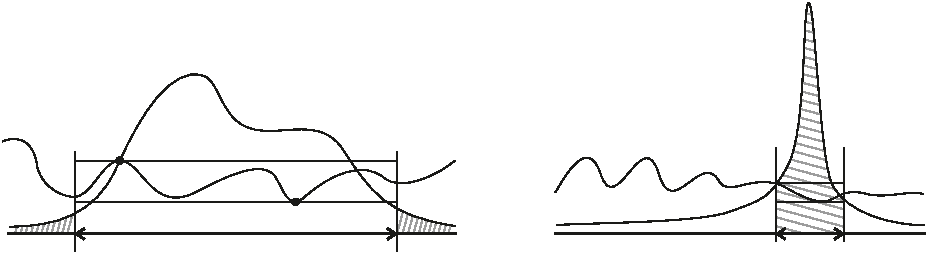
\includegraphics[width=15.0cm]{pictures/picture_4_1.pdf}};
	\draw [color=black](3,0.5) node[anchor=north west] {$ \delta $};
	\draw [color=black](0,-0.3) node[anchor=north west] {$ \theta $};
	\end{tikzpicture}
	\caption{popis}
\end{figure}
	
\end{remark}

\section{5.11.}
Problém principu neurčitosti: $\pi(\t)=$konst. na~$\Theta$ (rovnoměrnou apriorní informaci).
\begin{example}
	Mějme ÚBM, $X\sim f(x|\t),~\t\in(0,1),~\pi(\t)=1$ na~$(0,1)$. Bayes: $\pi(\t|\textbf{x})$.. $\widehat{\t}_B(\textbf{x})$. Označme $\eta=\t^2...,~\t=\sqrt{\eta}$, reparametrizace $f(x|\t=\sqrt{\eta})=f(x|\eta)$. $\t$ považujeme za~znáhodněné (apriorně předpokládáme, že o~$\t$ nic nevíme). Transformace hustoty, $\t$ na~$\eta$: $$\pi_H(\eta)=\pi(\sqrt{\eta})\cdot\big|\mathbb{J}_H(\eta)\big|=1\cdot\frac{1}{2\sqrt{\eta}}=\frac{1}{2\sqrt{\eta}}.$$
	Je paradoxní, že o~$\t$ nemáme konkrétní apriorní informaci a~přitom o~$\eta=\t^2$ víme, že (viz obr. \ref{fig:p71}) nevlastní.

\begin{figure}[h]
	\centering
	\begin{tikzpicture}
	\node[inner sep=0pt] (pic) at (0,0)
	{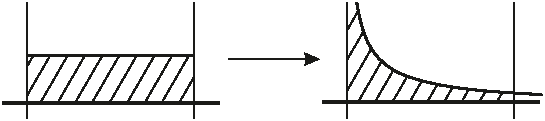
\includegraphics[width=12.0cm]{pictures/picture_4_2.pdf}};
	\draw [color=black](3,0.5) node[anchor=north west] {$ \delta $};
	\draw [color=black](0,-0.3) node[anchor=north west] {$ \theta $};
	\end{tikzpicture}
	\caption{popis}
\end{figure}

\end{example}
\begin{example}
	Mějme $X\sim f(x|\t),~\t\in\Theta,~\t\sim\pi(\t),~\mathcal{F}=\{f(x|\t)\}$. Zavedeme reparametrizaci $\eta=\inv{H}(\t)$, tzn. $\t=H(\eta)$. 
	$$ f_H(x|\eta)=f\big(x|\t=H(\eta)\big)=f\big(x|H(\eta)\big)...\mathcal{F}_H$$
	$$\pi(\t)\longrightarrow \pi_H(\eta)=\pi\big(H(\eta)\big)\cdot\big|D_H(\eta)\big| \text{, kde } D_H(\eta) \text{ je Jacobián.}  $$
	Z ÚBM $\{\mathcal{F},\pi\}$ plyne aposteriorní hustota $\pi(\t|\textbf{x})~\to~\widehat{\t}_B(\textbf{x})=\EE{\pi(\t|\textbf{x})}$. Dále z~ÚBM $\{\mathcal{F},\pi\}$ plyne ÚBM $\{\mathcal{F}_H,\pi_H\}$ a~z~něho aposteriorní hustota $\pi(\eta|\textbf{x})~\to~ \widehat{\eta}_B(\textbf{x})=\EE{\pi(\eta|\textbf{x})}$. 
	
	Pozor na~$\widehat{\t}_B\neq H(\widehat{\eta}_B)$! To může být problém.
\end{example}
\begin{theorem}[Jeffreys]
	Máme ÚBM $\mathcal{F},\pi(\t),~\eta=\inv{H}(\t),~\t=H(\eta)$ a~předpokládejme, že $\t\in\Theta\subset\R^k$ a~že $H$ je regulární transformace. Nechť $\mathcal{F}$ je regulární systém hustot ($\fregp$). Po reparametrizaci máme $\mathcal{F}_H,\pi_H$. Volme $\pi(\t)=\sqrt{\det \mathbb{J}(\t)}$, kde $\mathbb{J}(\t)$ je FIM pro~$\t$ v~$\mathcal{F}$. Pak $\pi_H(\eta)=\sqrt{\det \mathbb{J}_H(\eta)}$ v $\mathcal{F}_H$ a~platí, že 
	$$ \int_B\pi(\t|\textbf{x})\d\t=\int_{\inv{H}(B)}\pi_H(\eta|\textbf{x})\d\eta,\qquad\forall B\in\Bb_\Theta \text{ (B je borelovská množina).}$$
	\begin{proof}
		Pro $k=1$: (zbytek ponecháno čtenáři)\begin{enumerate}[a)]
			\item \[
			\begin{split}
			\int_B\pi(\t|\textbf{x})\d\t&=\frac{1}{c}\int_B f(\textbf{x}|\t)\pi(\t)\d\t=\left|\begin{array}{c}
			\t=H(\eta)\\D_H(\eta)
			\end{array}
			\right|=\frac{1}{c}\int_{\inv{H}(B)}\underbrace{f\big(\textbf{x}|H(\eta)\big)}_{f_H(\eta)}\underbrace{\pi\big(H(\eta)\big)\cdot\big|D_H(\eta)\big|}_{\pi_H(\eta)}\d\eta=\\&=\frac{1}{c_{(H)}}\int_{\inv{H}(B)}f_H\pi_H\d\eta=\int_{\inv{H}(B)}\pi(\eta|\textbf{x})\d\eta \hspace{0.3cm} (c \text{ a } c_{(H)} \text{ splývají}).
			\end{split}
			\]
			\item Protože 
			$$ \mathbb{J}_H(\eta)=\EE{\frac{\partial\log f_H(\eta)}{\partial\eta}}^2=\EE{\frac{\partial\log f(x|H(\eta))}{\partial\t}\frac{\partial H(\eta)}{\partial\eta}}^2=\mathbb{J}\big(H(\eta)\big) \cdot D_H^2(\eta) ,$$
			pak \[
			\begin{split}
			\pi_H(\eta)&=\pi\big(H(\eta)\big)\cdot\big|D_H(\eta)\big|=\sqrt{\det \mathbb{J}\big(H(\eta)\big)}\cdot\big|D_H(\eta)\big|=\sqrt{\det \mathbb{J}_H(\eta)D_H^{-2}(\eta)}\cdot\big|D_H(\eta)\big|=\\&=\sqrt{\det \mathbb{J}_H(\eta)}
			\end{split}
			\]
			Tedy $\pi(\t)=\sqrt{\det \mathbb{J}(\t)}$, což je \textbf{Jeffraysova apriorní hustota} (nebo také Jeffraysův princip neurčitosti).
		\end{enumerate}
	\end{proof}
\end{theorem}
Tedy pokud obecně o parametru $\t$ nevíme nic, tak máme 2 možnosti. Můžeme na celém oboru zvolit $\pi(\t)=1$, ale nebudeme mít zaručenou invarianci na reparametrizaci. Nebo právě můžeme zvolit Jeffraysovu apriorní hustotu, která často bývá nevlastní.
\begin{example}
	Mějme $X\sim f_X(x|\lambda)=\mathrm{Poiss}(\lambda)$, tzn. $f_{X_j}=\frac{\lambda^{x_j}}{x_j!}\e{-\lambda},~f_\textbf{x}(\textbf{x}|\lambda)=\frac{\lambda^{\sum x_j}}{\prod x_j!}\e{-n\lambda},~\lambda~>~0$.\begin{enumerate}[a)]
		\item Pokud je $\lambda$ neznámé, pak $\pi(\lambda)=1$ na~$\R^+$ (nevlastní). (Je jedno, jestli vezmeme rovno 1 nebo rovno nějaké konstantě.)
		$$
		\pi(\lambda|\textbf{x})=\frac{\fex \pi}{\underbrace{\int_{0}^{+\infty}\fex\pi\d\lambda}_{<+\infty}}=\underbrace{\frac{1}{c}\frac{1}{\prod x_j!}}_{\frac{1}{c'}}\lambda^{\sumjn x_j}\e{-n\lambda}\sim\mathrm{Gamma}\big(\sumjn x_j+1,n\big).$$
		
		Pro připomenutí: $\frac{1}{c'}x^{\alpha-1}e^{-\beta x}=\frac{\beta^{\alpha}}{\Gamma(\alpha)}x^{\alpha-1}e^{-\beta x } \sim \mathrm{Gamma}(\alpha,\beta) $
		
		Bayesovský odhad
		 $$\widehat{\lambda}_B=\EE{\mathrm{Gamma}(\underbrace{\sum x_j+1}_{\alpha},\underbrace{n}_\beta)}=\frac{\alpha}{\beta}=\frac{\sumjn x_j}{n}+\frac{1}{n}=\Oxn+\frac{1}{n}\sim \Oxn~(\text{MLE pro velká }n).$$
		\item Jeffrys: $$\pi(\lambda)=\sqrt{\det \mathbb{J}(\lambda)}=\sqrt{\det \EE{-\frac{\partial^2\log\fex}{\partial\lambda^2}}}=\sqrt{n\cdot\frac{1}{\lambda}}=\sqrt{n}\frac{1}{\sqrt{\lambda}}.$$
		Volba $\pi(\lambda)=\frac{1}{\sqrt{\lambda}}$ viz obr. \ref{fig:p72} (V apriorní informaci nehraje konstanta roli, protože se vždy v Bayesově vzorci pokrátí, tedy můžeme vypustit $\sqrt{n}$).
		\begin{figure}[h]
			\centering
			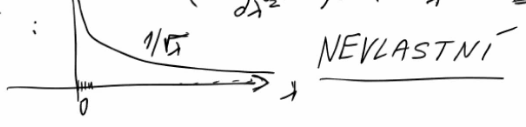
\includegraphics[width=0.5\linewidth]{pictures/P7_2}
			\caption{Nevlastní}
			\label{fig:p72}
		\end{figure}
		$$ \pi(\lambda|\textbf{x})=\frac{f \pi(\lambda)\cancel{c}}{\underbrace{\int f\pi(\lambda)\cancel{c}\d\lambda}_{<+\infty}}=\frac{1}{c'}\lambda^{\sumjn x_j-\frac{1}{2}}\e{-n\lambda}\sim\mathrm{Gamma}\Big(\underbrace{\sumjn x_j+\frac{1}{2}}_{\tilde{\alpha}},\underbrace{n}_{\tilde{\beta}}\Big).$$
		Bayesovský odhad $\widehat{\lambda}_B^J=\EE{\mathrm{Gamma}(\tilde{\alpha},\tilde{\beta})}=\frac{\tilde{\alpha}}{\tilde{\beta}}=\Oxn+\frac{1}{2n}\sim\Oxn$ (MLE pro velká $n$).
	\end{enumerate}
	Pro $n$ malá se odhady v a) a b) liší.
\end{example}

\section{Limitní aposteriorní hustoty ($\widehat{\t}_B$)}
Mějme ÚBM $\{\mathcal{F},\pi(\t)\}$ a~předpokládejme, že $\pi\in\Pi=\{\pi(\t,\boldsymbol{\lambda}):\boldsymbol{\lambda}\in\Lambda\}=\mathcal{H}$. Volme $\lambda_0\in\partial\Lambda$ z hranice a~definujme limitní apriorní hustotu $\pi_{\lambda_0}(\t)=\lim\limits_{\substack{
		\lambda\to\lambda_0\\\lambda\in\Lambda	}
}c\cdot \pi(\t,\lambda)$, která bývá často nevlastní. 

Dále pak vyjádříme limitní aposteriorní hustota (za předpokladu záměny integrálu a~limity v parametrickém integrálu) $$\pi_{\lambda_0}(\t|\textbf{x})\equal{ozn}\frac{f\pi_{\lambda_0}(\t)}{\int_\Theta f\pi_{\lambda_0}(\t)\d\t}=\frac{f\lim\limits_{\lambda\to\lambda_0}c\pi(\t,\lambda)}{\int_\Theta f\lim\limits_{\lambda\to\lambda_0}c\pi(\t,\lambda) \d\t}=\lim\limits_{\substack{
		\lambda\to\lambda_0\in\partial\Lambda\\\lambda\in\Lambda	}
}\frac{f\pi(\t,\lambda)}{\int f\pi(\t,\lambda)\d\t}=\lim\limits_{\lambda\to\lambda_0}\pi(\t|\textbf{x},\lambda).$$
Z toho vyplývá, že $\htb^\mathrm{lim} =\EE{\pi_{\lambda_0}(\t|\textbf{x})}$, což často vede na~nějakou~klasickou statistickou proceduru.

\begin{example}
	Mějme $X\sim f_X=\mathrm{Exp}(\t),~f_X=\theta\e{-\t x},~\t>0$, $$\mathcal{H}=\{\t\sim\mathrm{Gamma}(\alpha,\beta),~\text{tzn. }\pi\big(\t,\underbrace{(\alpha,\beta)}_{\boldsymbol{\lambda}}\big)=\t^{\alpha-1}\e{-\beta\t}\},~\Lambda=\R^{2+}.$$ $\boldsymbol{\lambda}_0=(0,0)\in\partial\Lambda\Rightarrow\pi_{0,0}(\t)=\lim\limits_{(\alpha,\beta)\to(0,0)^{+}}\t^{\alpha-1}\e{-\beta\t}=\frac{1}{\t}$ (nevlastní).
	$$\pi_{(0,0)}(\t|\textbf{x})=\frac{f\cdot\frac{1}{\t}}{\underbrace{\int_{0}^{+\infty}f\cdot\frac{1}{\t}\d\t}_{<+\infty}}\equal{iid}\frac{\t^n e{-\t\sumjn x_j}\cdot\frac{1}{\t}}{c}=\frac{1}{c}\t^{n-1}\e{-\t\sumjn x_j}\sim\mathrm{Gamma}\Big(n,\sumjn x_j\Big),$$
	$$\htb^{\mathrm{lim}}=\E\Big[\mathrm{Gamma}\Big(n,\sumjn x_j\Big)\Big]=\frac{n}{\sumjn x_j}=\inv{(\Oxn)}=\html.$$
	Pokud bychom chtěli dostat pouze $\Oxn$, tak bychom v $\mathcal{H}$ museli namísto $\mathrm{Gamma}$ rozdělení použít inverzní $\mathrm{Gamma}$ rozdělení.
\end{example}
\begin{example}
	Volba $\pi(\t)$? Subjektivní. New England Journal of Medicine - studie\begin{enumerate}[1)]
		\item léčba rakoviny plic - operace - víme, že šance na~přežití je 68\%, ale jen 44\% lidí by tam šla. 
		\item léčba rakoviny plic - operace - víme, že pravděpodobnost úmrtí je 32\%, ale jen 18\% lidí by tam šla. 
	\end{enumerate}
\end{example}

\subsection{Empirical Bayes}
Máme $\mathcal{H}=\{\pi(\t,\lambda):\lambda\in\Lambda\}$. Spočítá se marginální rozdělení $m_\lambda(\textbf{x})=\int_\Theta\underbrace{f(\textbf{x}|\t)\pi(\t,\lambda)}_{\phi(\textbf{x},\t,\lambda)}\d\t$. Vezmete data $\textbf{X}$, realizace $\textbf{x}$ a  na~základě dat odhadneme klasickou statistickou procedurou (např. $\lambda_{ML}$ - maximálně věrohodný odhad) $\widehat{\lambda}(\textbf{x})$ v~té $m_\lambda(\textbf{x})$ a~provedeme Bayesovský princip s~apriorní hustotou $\pi(\t,\widehat{\lambda}_{\mathrm{ML}})$ klasickou statistickou procedurou $\widehat{\lambda}_{\mathrm{ML}}$.

Principem ME $H(\pi)=-\int_\Theta\pi(\t)\log \pi(\t)\d\t$ .. $\pi$ volíme tak, aby $H(\pi)$ bylo maximální.

%%%%%%%%%%%%%%%%%%% lesson 8

Máme tedy omezení ve formě $\E^\pi[g_i(\t)]=\omega_i,~\forall i\in K$. $H(\pi)$ max vazebné je $$\pi^K(\t_i)=\frac{\e{\sumjn \lambda_j g_j(\t_i)}}{\sum \e{\sumjn \lambda_jg_j(\t_i)}},~\forall i,$$
kde $\lambda_j$ jsou Lagrangeovy koeficienty.

$$ KL(\pi,\pi_0)=\E^\pi\big[\log\frac{\pi_0}{\pi}\big]=\int\pi\log\frac{\pi_0}{\pi}\d\t.$$
Pokud $\pi_0=1$, pak $KL(\pi,1)=-\int\pi\log\pi=H(\pi)$. Závisí naše volba $\pi$ na $\pi_0$?

\begin{define}[Konjugované sytémy apriorní hodnoty]
	Mějme systém hustot $\mathcal{F}=\{f(x|\t):\t\in\Theta\subset\R^k\}$ a označme $\mathcal{H}$ systém hustot pro $\t$. $\mathcal{H}$ nazveme \textbf{konjugovaný sytém apriorní hodnoty} pro $\mathcal{F}$, pokud $\pi(\t|\textbf{x})\in\mathcal{H}$.
\end{define}
\begin{theorem}
	Mějme $\mathcal{F}_n=\{\fex(\textbf{x}|\t)=\prod_{j=1}^n f_{X_j}(x_j|\t)\} ~id$ a předpokládejme, že $T_n(\textbf{X})$ je postačující statistika pro $\mathcal{F}_\textbf{X}$, tzn. dle Neymannova faktorizačního kritéria $\fex(\textbf{y}|\t)=h_n(\textbf{y})g_n\big(T_n(\t,\textbf{y})\big),$ $\forall\t,\forall\textbf{y},\forall n$. Pak $$\mathcal{H}=\bigg\{\frac{g_m(\boldsymbol{\t},\textbf{t})}{\int g_m(\boldsymbol{\t},\textbf{t})\d\t}:\forall m\in\N,\forall\textbf{t}\in S_m,\text{ kde }S_m=\{\textbf{t}:\exists\textbf{y},\text{ že }T_m(\textbf{y})=\textbf{t}\}\bigg\}\text{ je CF.}$$
	\begin{proof}
		$\pi(\t)\in\mathcal{H}$, tzn. $\pi(\t)\sim g_m(\t,\textbf{t})$. Z toho vyplývá, že $\exists\textbf{y}$ tak, že $T_m(\textbf{y})=\textbf{t}$. Dále pak platí, že \[
		\begin{split}
		\pi(&\t|\underbrace{\textbf{x}}_{\dim n})\sim f_n(\textbf{x}|\t)g_m(\boldsymbol{\t},\textbf{t})\sim \underbrace{g_m\big(\t,T_m(\textbf{y})\big)h_m(\textbf{y})}_{NF_nK\Rightarrow f_m(\textbf{y}|\t)}f_n(\textbf{x}|\t)=f_m(\textbf{y}|\t)f_n(\textbf{x}|\t)=\\&=\prod_{j=1}^mf(y_j|\t)\prod_{j=1}^nf(x_j|\t)=\prod_{j=1}^{m+n}\underbrace{f_{Z_j}(z_j|\t)}_{\textbf{z}=(\textbf{y},\textbf{x})}=f_{m+n}(\textbf{z}|\t)=\underbrace{h_{n+m}(\textbf{z})}_{\text{konst}}g_{n+m}\big(\t,\underbrace{T_{n+m}(\textbf{y})}_{\textbf{t}\in S_{n+m}}\big)\sim g_{n+m}(\t,\textbf{t})
		\end{split}
		\]
		Z rozšíření na $m\in\R$ (vhodně) vznikne CF (obvyklá).
	\end{proof}
\end{theorem}
\begin{example}
	Mějme $X\sim f_X(x|\t)=\Exp(\lambda)$, $f_X=\lambda\e{-\lambda x},~\lambda>0$. $$\mathcal{F}_n: ~f_n(\textbf{x}|\underbrace{\t}_{\lambda})=\lambda^n\e{-\lambda\sumjn x_j}=\left|\begin{array}{c}
	ozn.~T_n(\textbf{x})=\sumjn x_j\\\text{je PS pro }\mathcal{F}_n
\end{array}
\right|=1\cdot g_n\big(\lambda,T_n(\textbf{x})\big).$$
Označme $$\sumjn x_j=t~\Rightarrow~\mathcal{H}=\Big\{ \frac{g_m(\lambda,\textbf{t})}{c}:m\in\N,~t\in S_m,... \Big\}=\Big\{\underbrace{\lambda^m\frac{\e{-\lambda t}}{c}}_{\Gamma(m+1,t)}:m\in\N,t\in S_m=\{\textbf{t}=\sum x_j \}=\R^+\Big\}.$$
Přirozená CF ... širší $\Gamma(\alpha,\beta)=\Hobv ,~\alpha,\beta>0$.
Protože $X\sim\Exp(\lambda),~\pi(\lambda)=\mathrm{Gamma}(\alpha,\beta)$, pak 
$$ \pi(\lambda|\textbf{x})=\frac{\lambda^n\e{-\lambda\sum x_j}\frac{1}{c}\lambda^{\alpha-1}\e{-\lambda\beta}}{\int_{0}^{+\infty}\lambda^n\e{-\lambda\sum x_j}\frac{1}{c}\lambda^{\alpha-1}\e{-\lambda\beta}\d\lambda}=\frac{\lambda^{n+\alpha-1}\e{-\lambda(\sum x_j+\beta)}}{c}\sim\mathrm{Gamma}\big(n+\alpha,\sumjn x_j+\beta\big)\in\Hobv .$$

Seznam CF: \begin{enumerate}[a)]
	\item $X\sim \mathrm{Bi}(n,p)\Rightarrow CF~\mathcal{H}=\{\pi(p)\sim\mathrm{Beta}(\alpha,\beta)\}$,
	\item $X\sim\mathrm{Poisson}(\lambda)\Rightarrow CF~\mathcal{H}=\{\pi(\lambda)\sim\mathrm{Gamma}(\alpha,\beta)\}$,
	\item $X\sim U(0,\t),~\t\in\R^+\Rightarrow CF~\mathcal{H}=\{\pi(\t)\sim\mathrm{Pareto}(a,b)\}$, kde Paretovo rozdělení je mocninného typu $\t\sim\frac{a}{b}\big(\frac{b}{\t}\big)^{a+1},~\t\geq b$, které má těžké chvosty.
	\item \begin{enumerate}[1)]
		\item $X\sim \NN(\mu,\sigma_0^2),~\sigma_0\text{ známé }>0$, pak PS je ve tvaru $T_n(\textbf{X})=\sumjn X_j\in\R$. Potom $$\HCF=\big\{\pi(\mu)\sim\NN(a,b^2),~a\in\R,b>0\big\}$$ a parametry $a,b$ ladíme pro tvar apriorní informace.
		\item $X\sim\NN(\mu_0,\sigma^2),~\mu_0$ známe. Pak PS je ve tvaru $T_n(\textbf{X})=\sumjn(X_j-\mu_0)^2$, protože 
		$$ \fex=\underbrace{\frac{1}{c}\e{-\frac{1}{2\sigma^2}\sumjn(X_j-\mu_0)^2}}_{g_n(t,\sigma^2)},$$ a proto $\Hobv$ pro parametr $\underbrace{\frac{1}{\sigma^2}}_{\t}=\{\pi(\t)\sim\mathrm{Gamma}(\alpha,\beta)\}.$
		\item $X\sim\NN(\mu,\sigma^2)$. Pak $\pi_n(\textbf{X})=\Big(\sumjn X_j,\sumjn X_j^2\Big)\in\R\times\R_0^+$ je PS, a proto
		$\Hobv$ pro $(\mu,\frac{1}{\sigma^2})$ definujeme tak, že $\pi\big(\mu\frac{
		1}{\sigma^2}\big)\sim\NN$ a $\pi\big(\frac{1}{\sigma^2}\big)\sim\mathrm{Gamma}$. Z toho pak 
		$$ \pi\big(\mu,\frac{1}{\sigma^2}\big)=\pi\big(\mu|\frac{1}{\sigma^2}\big)\pi\big(\frac{1}{\sigma^2}\big)=N\cdot\mathrm{Gamma}.$$
	\end{enumerate}
\end{enumerate}
\end{example}
\begin{remark}
	$\pi(\t)=\sum_{i=1}^lw_i\pi_i(\t)$, kde $\pi_i\in\HCF$. Pak $$\pi(\t|\textbf{x})=\frac{f\pi}{\int f\pi}=\frac{1}{c}\sum_{i=1}^lw_i f\pi_i(\t)=\frac{1}{c}\sum_{i=1}^l w_ic_i\frac{f \pi_i}{c_i~(=\int f\pi_i\d\t)}=\sum_{i=1}^l \underbrace{\frac{w_ic_i}{c}}_{w_i'}\pi_i(\t|\textbf{x})=\sum_{i=1}^l w_i\underbrace{\pi_i(\t|\textbf{x})}_{\HCF}.$$
		\begin{figure}[h]
			\centering
			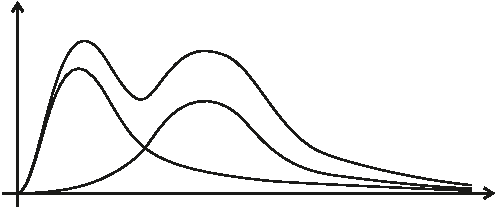
\includegraphics[width=0.6\linewidth]{pictures/8_1.pdf}
			\caption{no idea what is it and where did it come from :D....me neither :D}
			\label{fig:81}
		\end{figure}
		
\end{remark}

\section{Propojování Bayese s klasickou statistikou (nejméně příznivost)}
\begin{define}
	Mějme $\t\in\Theta,~\tau(\t)\in\mathcal{T},~\mathscr{D},~L(\t,\delta)$ ztrátu, $\RF(\t,\delta)$ riziko $=\E^fL,~\sup_\t\RF(\t,\delta)$. ÚBM: $r(\pi,\delta)=\E^\pi\RF(\t,\delta)$.. $\delta_{(B)}^\pi$. Definujeme $\RF=\sup\limits_{\pi\in\Pi}r(\pi,\delta^\pi)=\sup\limits_{neco}r(\pi),$ kde $\Pi$ je rodina apriorních hustot a $\RF$ nazveme riziko.
\end{define}
\begin{theorem}\label{veticka}
	$\underline{\RF}\leq \overline{\RF}$, kde $\overline{\RF}=\inf\limits_\delta\sup\limits_\t \RF(\t,\delta)$ (minimální riziko).
	\begin{proof}
		$\pi$ apr.r. (nevím), a proto $$ r(\pi,\delta)=\int_\Theta\underbrace{\RF(\t,\delta)}_{\geq0}\underbrace{\pi(\t)}_{\geq0}\d\t\leq \int\sup\limits_\t \RF(\t,\delta)\pi(\t)\d\t=\sup\limits_\t \RF(\t,\delta)\cdot 1.$$
		Dále platí nerovnice \[
		\begin{split}
		r(\pi,\delta)&\leq \sup\limits_\t\RF(\t,\delta),\quad \forall\delta,\forall\pi\\
		\inf\limits_\delta r(\pi,\delta)&\leq \inf\limits_\delta\sup\limits_\t \RF (=\overline{\RF}),\quad \forall\pi\\
		\sup\limits_\pi\inf\limits_\delta r=\underline{\RF}&\leq \overline{\RF}
		\end{split}
		\]
	\end{proof}
\end{theorem}
\begin{remark}
	Pokud $\delta^\pi$ dosahuje na $\underline{\RF}$ a $\underline{\RF}=\overline{\RF}$ ve větě \ref{veticka}, pak $\delta^\pi$ je současně \textbf{minimaxní strategie}.
\end{remark}
\begin{define}
	Pokud existuje $\pi^\ast$ apriorní rozdělení, že $r(\pi ^\ast)=\RF$ (tzn. $\forall\pi\in\Pi,~r(\pi)\leq r(\pi^\ast)$), tak pak se nazývá \textbf{nejméně příznivé} (least favourable).
\end{define}

\begin{theorem}
	Nechť $\pi$ je vlastní apriorní r. na $\Theta$ tak, že $r(\pi)=\sup\limits_\t\RF(\t,\delta^\pi)$. Pak \begin{enumerate}
		\item $\delta^\pi$ je MINIMAX,
		\item $\delta^\pi$ jedn. Bayes, pak $\delta^\pi$ je jedn. MIMAX,
		\item $\pi$ je LF. 
	\end{enumerate}
\begin{proof}
	\begin{enumerate}
		\item $\delta$ libovolné fixní. Pak $\sup\limits_\t\RF(\t,\delta)\geq\int\RF\pi(\t)\d\t=\E^\pi\RF=r(\pi,\delta)\geq r(\pi,\delta^\pi)=r(\pi)=\sup\limits_\t\RF(\t,\delta^\pi)$.
		\item $>$
		\item $\pi'$ libovolné fixní. Pak $r(\pi')=r(\pi',\delta^{\pi'})\leq r(\pi'\delta^\pi)\leq \sup\limits_\t\RF(\t,\delta^\pi)=r(\pi)$. Potom $\pi$ ($=\pi^\ast$) je LF.
	\end{enumerate}
\end{proof}
\end{theorem}
\begin{dusl}
	V ok, pokud $\RF(\t,\delta^\pi)$ je konstantní v $\t$ na $\Theta$ $s.j.\pi$, tedy $r(\pi)=\sup\RF$.
\end{dusl}
\begin{theorem}
	Nejméně příznivá posloupnost $(\pi_n)_1^{+\infty}$ je taková, že $\lim\limits_{n\to+\infty} r(\pi_n)=\RF$. 
\end{theorem}
\begin{theorem}
	Nechť $(\pi_n)_1^{+\infty}$ je taková posloupnost, že $\lim\limits_{n\to+\infty}r(\pi_n)=r$. Nechť $\delta_0$ je rozhodovací funkce taková, že $\sup\limits_\t \RF(\t,\delta_0)=r$. Pak \begin{enumerate}
		\item $\delta_0$ je minimax,
		\item X
		\item $(\pi_n)_1^{+\infty}$ je LF
	\end{enumerate}
\begin{proof}
	Analogicky jako v \ref{veticka} (tedy za domácí cvičení).
\end{proof}
\end{theorem}
\begin{remark}
	Mějme $X\sim \mathrm{Bi}(n,p),~\widehat{p}=?,~\pi(p)\sim\mathrm{Beta}(a,b)\sim\frac{1}{B(a,b)}p^{a-1}(1-p)^{b-1}$. Příkladem může být teorie spolehlivosti, kde máme datové pole v RAIDu, tj. $n$ komponentní systém. Označme $X$ počet poruch za čas $1$. $\{X\geq5\}\Rightarrow$ výpadek. Jaká je pravděpodobnost $\PP(X\geq5)=\widehat{p}$. $\widehat{\E X}=n\widehat{p}$ za čas 1.
	
	Se zadáním můžeme dělat několik věcí:\begin{enumerate}[1)]
		\item apriorní odhad $\widehat{p}_a=\E\mathrm{Beta}(a,b)=\frac{a}{a+b}.$
		\item Můžeme naměřit data $x$ a vypočíst klasický ML: $\widehat{p}_\mathrm{ML}=\frac{x}{n}=\oxnn ... \widehat{p}_\mathrm{UMVUE}$ $(L=L_2)$.
		\item Bayesovský odhad: $$\pi(p|x)=\frac{\binom{n}{x}p^x(1-p)^{n-x}\cdot\frac{1}{B(a,b)}p^{a-1}(1-p)^{b-1}}{\int_{0}^{1}...\d p}=\frac{1}{c}p^{x+a-1}(1-p)^{n-x+b-1}\sim\mathrm{Beta}(x+a,n-x+b).$$
		Z toho potom $\widehat{p}_B=\E \mathrm{Beta}(x+a,n-x+b)=\frac{x+a}{n+a+b}=\frac{\oxnn+\frac{a}{n}}{1+\frac{a+b}{n}}$. Zároveň však
		$$ \widehat{p}_B=\frac{a+b}{a+b+n}\frac{a}{a+b}+\frac{n}{n+a+b}\frac{x}{n}==\alpha_n\widehat{p}_a+(1-\alpha_n)\widehat{p}_\mathrm{ML}.$$
		\begin{enumerate}[a)]
			\item $n$ pevně, $a,b\to+\infty$ (velké), $b/a=konst$ $(\alpha_n\to1\Rightarrow\widehat{p}_B=\widehat{p}_a)$
			\item $a,b$ pevně, $n\to+\infty$ (velké), pak $\alpha_n\to0$ $(\alpha_n\doteq0)\Rightarrow\widehat{p}_B=\widehat{p}_\mathrm{ML}$,
			\item $a=b=1$, tzn. $\pi(p)=U(0,1)$ princip neurčitosti. Z toho pak $\widehat{p}_B=\frac{x+1}{n+2}\doteq \widehat{p}_\mathrm{ML}$ pro vysoká $n$.
			\item $a=b=0,~\pi(p)=\inv{p}\inv{(1-p)}$ nevlastní (limitní), pak $\pB=\pML$.
			\item $a=a_n=\frac{\sqrt{n}}{2},~b=b_n=\frac{\sqrt{n}}{2}$, tzn. $\pi(p)=\mathrm{Beta}\big(\frac{\sqrt{n}}{2},\frac{\sqrt{n}}{2}\big)$ (závisí na $n$).
			\[
			\begin{split}
			\pB&=\frac{x+\frac{\sqrt{n}}{2}}{n+\sqrt{n}}\Rightarrow \RF(p,\pB)=\Big|L=L_2\Big|=\E \underbrace{(p-pB)^2}_{L_2(p,\pB)}=\E\Big(p-\frac{X+\frac{\sqrt{n}}{2}}{n+\sqrt{n}}\Big)^2=\\&=c\underbrace{\E X^2}_{np-np^2+n^2p^2}+d \underbrace{\E X}_{np}+e\equal{...}\frac{n}{4(n+\sqrt{n})^2}=konst.
			\end{split}
			\] 
			Dle V víme, že $r(\pi)=\sup\limits_{\theta}\RF(\t,\delta^\pi)$ implikuje to, že $\pB=\widehat{p}_\mathrm{Minimax}$ a $\pi^\ast=\pi(p)$ je LF.
			\begin{figure}[h]
				\centering
				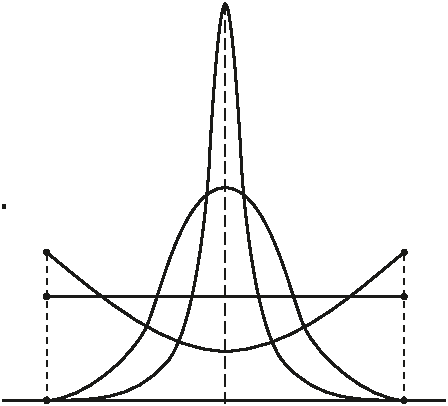
\includegraphics[width=0.5\linewidth]{pictures/9_1.pdf}
				\caption{popis}
				\label{fig:91}
			\end{figure}			
		\end{enumerate}
	\end{enumerate}
\end{remark}	
	
\begin{remark}
	Mějme $X\sim\NN(\mu,1)=\NN(\t,1),~\wmu=?$ a\begin{enumerate}[A)]
		\item $\pi(\mu)=konst=1$ na $\R$ nevlastní, tedy $\wmu_a$ není. $$\pi(\mu|x)=\frac{1}{\sqrt{2\pi}}\e{-\frac{1}{2}(x-\mu)^2}\cdot \frac{1}{\int_\R...\d\mu}=\frac{1}{\sqrt{n}}\e{-\frac{1}{2}(\mu-x)^2}\sim\NN(x,1).$$
		$$\widehat{\mu}_B=\EE{\NN(x,1)}=x(=\oxnn),$$
		$$ \RF(\mu,\widehat{\mu}_B)\equal{L=L_2}\E(\mu-X)^2=\D X=1~konst,\text{ ale nelze aplikovat tu V...}$$
		\item $\pi_n(\mu)=\NN(0,n)$ vlastní $\forall n$ (CF).
		\[
		\begin{split}
		\pi_n(\mu|x)~\propto~ \e{-\frac{1}{2}(x-\mu)^2}\e{-\frac{1}{2n}(\mu-0)^2}~\propto~\e{-\frac{1}{2}\big[\big(1+\frac{1}{n}\big)\mu^2-2\mu x+x^2\big]}~\propto~\e{-\frac{1}{2}\big(1+\frac{1}{n}\big)\big[\mu-\frac{n}{n+1}x\big]^2}\sim \NN\Big(\frac{n}{n+1}x,\frac{n}{n+1}\Big)
		\end{split}
		\]
		$$\widehat{\mu}_B=\E \NN\Big(\frac{n}{n+1}x,\frac{n}{n+1}\Big)=\frac{n}{n+1}x=\delta^{\pi_n}\sim\widehat{\mu}_{B,n}.$$
		$$r(\pi_n)\equal{L=L_2}\D \pi(\mu|x)=\frac{n}{n+1}\to1.$$
		$\lim\limits_{n\to+\infty}r(\pi_n)=1=r$ a víme, že 
		----nestihl jsem to, konec strany
	\end{enumerate}
\end{remark}
\begin{theorem}[Vyhazovací]
	ÚBM $X\sim f(x|\t),~\pi(\t),~L(\t,\delta)=L_2(\t,\delta)=(\t,\delta)^2$. Nechť $0<\E^\pi(\t^2|x)<+\infty$. Pak $$\delta^\pi(x)=\E^\pi(\t|x)=\frac{\int\t f(x|\t)\pi(\t)\d\t}{\int f(x|\t)\pi(\t)\d\t}$$
	a pro Bayesovské riziko 
	$$r(\pi)=\E^m[\D^\pi(\t|x)],$$
	kde $m(x)=\int f\pi\d\t$.
	\begin{proof}
		\[
		\begin{split}
		\delta^\pi&=\argmin\limits_{\delta} r(\pi,\delta),~r(\pi,\delta)=\E^\pi[\RF(\t,\delta)]=\E^\pi\big[\E^f\big(\t-\delta(X)\big)\big]=\left|\begin{array}{c}
		\text{záměna} \\ \E^\pi\text{ a }\E^f		
		\end{array}
		\right|=\E^m\big[\E^\pi\big(\t-\delta(x)\big)^2\big|x\big]=\\&=\E^m\big[\E^\pi(\t^2|x)-2\delta(x)\E^\pi(\t|x)+\delta(x)^2\big]=\E^m\big[\underbrace{\E^\pi(\t^2|x)}_{0<...<+\infty}+\big(\delta(x)-\E^\pi(\t|x)\big)^2-\underbrace{\big(\E^\pi(\t|x)\big)^2}_{0<...<+\infty}\big]
		\end{split}
		\] Abychom tento výraz optimalizovali, musíme vzít $\delta(x)=\E^\pi(\t|x)$, abychom výraz minimalizovali.
		$$ r(\pi)=r(\pi,\delta^\pi)=\E^m\big[\underbrace{\E^\pi\big(\t-\E^\pi(\t|x)\big)^2|x}_{\D(\t|x)}\big].$$
	\end{proof}
\end{theorem}

\section{Přípustnost (Admissibility)}
\begin{define}
	Mějme $\mathscr{D},\Theta,...$ Rozhodovací funkce $\delta_0$ se nazývá \textbf{nepřípustná}, pokud existuje $\delta_1$ která dominuje $\delta_0$, ozn. $\delta_1\ll\delta_0$, tzn. $\RF(\t,\delta_1)\leq\RF(\t,\delta_0),~\forall\t\in\Theta$ (stejnoměrně) a $\exists\t_0$ tak, že $\RF(\t_0,\delta_1)<\RF(\t_0,\delta_0)$. V případě, že taková $\delta_1$ neexistuje, pak $\delta_0$ nazýváme \textbf{přípustný}.
	
	\begin{figure}[h]
		\centering
		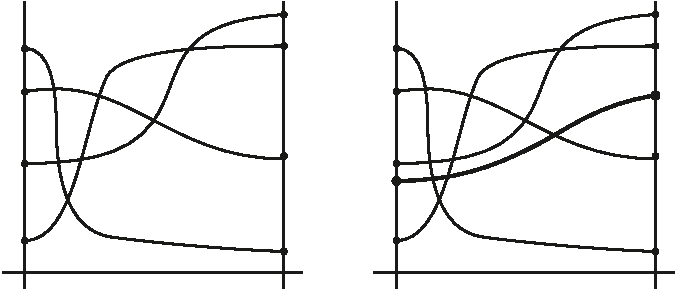
\includegraphics[width=0.6\linewidth]{pictures/9_2-3.pdf}
		\caption{Který je přípustný? Všechny 4. Vpravo ale už je $\RF(\t,\delta_\circ)$ nepřípustný.}
		\label{fig:92}
	\end{figure}
	
\end{define}
\begin{theorem}
	\begin{itemize}
		\item 
	$\delta_L(x)=\argmin\limits_\delta L\big(\t,\delta(x)\big),~\forall\t,\forall x$, je vždy přípustný, pokud existuje, \item  $\delta_u=\argmin\limits_\delta\RF(\t,\delta),~\forall\t$, je vždy přípustný, pokud existuje, \item  $\delta_0=\argmin\limits_\delta\sup\limits_\t\RF(\t,\delta),~\forall\t$, je přípustný, pokud existuje a je jednoznačný, \item  $\delta^\pi=\argmin\limits_\delta r(\pi,\delta)$ je přípustný, pokud existuje a je jednoznačný.
\end{itemize}
\end{theorem}


%%% 26.11.2020

\begin{theorem}
	Nechť $L(\t,\delta)$ je striktně konvexní v $\delta$ pro $\forall\t$. Mějme $\delta_0$ rozhodovací funkci pro $\tau(\t)|(\t)$ a $\delta_0$ je přípustný. Nechť $\delta'$ je tak, že $\RF(\t,\delta')=\RF(\t,\delta_0),~\forall\t$. Pak $\delta'=\delta_0$ s pravděpodobností 1 ($s.j.$), tedy $$ \E L(\t,\delta'(X))=\E\big(L(\t),\delta_0(X)\big).$$
	\begin{proof}
		Sporem: $\delta_0\neq\delta'$ s nenulovou pravděpodobností. Sestrojíme $\delta^\ast=\frac{\delta_0+\delta'}{2}$ konvexní. Pak
		\[
		\begin{split}
		\RF(\t,\delta^\ast)&=\E L\big(\t,\delta^\ast(X)\big)=\E\Big[L\Big(\t,\frac{\delta_0+\delta'}{2}\Big)\Big]<\E\Big[\frac{1}{2}L(\t,\delta_0)+\frac{1}{2}L(\t,\delta')\Big]=\\&= \frac{1}{2}\underbrace{\E L(\t,\delta_0)}_{\RF(\t,\delta_0)}+\frac{1}{2}\underbrace{\E L(\t,\delta')}_{\RF(\t,\delta')=\RF(\t,\delta_0\forall\t)}=\RF(\t,\delta_0),~\forall\t.
		\end{split}
		\] 
		To znamená, že $\delta^\ast\ll\delta_0$, což je spor s přípustností $\delta_0$.
	\end{proof}
\end{theorem}
\begin{theorem}
	Jednoznačná $\delta^\pi$ je vždy přípustná riziková funkce.\begin{proof}
		$\delta^\pi$ jednoznačný Bayes, pak \[
		\begin{split}
		r(\pi,\delta^\pi)&<r(\pi,\delta),\quad\forall\delta,\\
		\E \RF(\t,\delta^\pi)&<\E \RF(\t,\delta),\quad\forall\delta,\\
		\int\RF(\t,\delta^\pi)\pi(\t)\d\t&<\int\RF(\t,\delta)\pi(\t)\d\t,\quad\forall\delta.		
		\end{split}
		\]
		Z toho vyplývá, že $\exists\t_0$, $\RF(\t_0,\delta^\pi)<\RF(\t_0,\delta),~\forall\delta$. Kvůli tomu $\delta$ nedominuje $\delta^\pi$, a proto je $\delta^\pi$ přípustná.
	\end{proof}
\end{theorem}
\begin{remark}
	Pokud $L(\t,\delta)$ je striktně konvexní v $\delta$ pro $\forall\t$, pak $\delta^\pi$ je vždy jednoznačná.
\end{remark}
\begin{theorem}
	ÚBM $f,~\pi(\t)$. Nechť $\pi(\t)>0$ pro $\forall\delta$. Pak $\delta^\pi$ je přípustná.
	\begin{proof}
		Sporem. Nechť $\delta^\pi$ je nepřípustná. Pak by ale $\exists\delta_0\ll\delta^\pi$, tzn. $\RF(\t,\delta_0)$ stejnoměrně vylepšuje $\RF(\t,\delta^\pi)$ a $\exists\t_0$ tak, že $\RF(\t_0,\delta_0)<\RF(\t_0,\delta^\pi)$,viz obr. \ref{fig:26}.
		\begin{figure}[h]
			\centering
			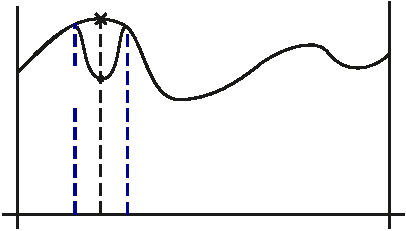
\includegraphics[width=0.35\linewidth]{pictures/26_11.pdf}
			\caption{popis}
			\label{fig:26}
		\end{figure}
		Potom by ale existovalo $H_{\t_0}$ tak, že $\RF(\t,\delta_0)<\RF(\t,\delta^\pi)$ na $H_{\t_0}$. Potom by platilo, že $\E \RF(\t,\delta_0)<\E^\pi \RF(\t,\delta^\pi)$. To platí, protože $\pi(\t)>0,~\forall\t$. Potom tedy 
		$$ r(\pi,\delta_0)<\underbrace{r(\pi,\delta^\pi)}_{r(\pi)<+\infty},$$ což je spor s Bayesem.
	\end{proof} 
\end{theorem}
\begin{remark}
	$\pi(\t)>0$
\begin{enumerate}[a)]
	\item 	\begin{center}
			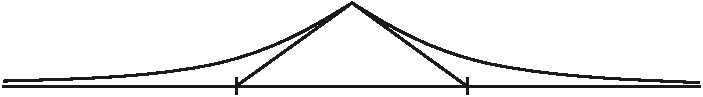
\includegraphics[width=0.7\linewidth]{pictures/26_11_2.pdf}
	\end{center}
\item $\RF(\t,\delta)=\E L\big(\t,\delta(X)\big)=\int_{\chi(\R^n)}L\big(\t,\delta(x)\big)f(x|\t)\d x$. Zde stačí zajistit, aby měl integrand Lebegovskou majorantu.
\end{enumerate}

\end{remark}
\begin{remark}
	$\delta^\pi$ podmiňuje přípustnost.\begin{description}
		\item[Stein (1955+)] Nutnou a postačující podmínkou, za které jsou všechny přípustné riziková funkce limitami posloupnosti $\delta^{\pi_m}$ Bayesovskou strategií.
		\item[Farrell (1968)] Předpokládáme, že \begin{enumerate}[1)]
			\item $f(x|\t)$ spojitá v $\t$, $f>0$ na $\Theta$,
			\item $L(\t,\delta)$ je striktně konvexní, spojitá,
			\item $\forall E\subset\Theta$ kompaktní platí, že 
			$$ \lim\limits_{\left\|\delta\right\|\to+\infty}\inf\limits_{\t\in E}L(\t,\delta)=+\infty.\qquad(\text{L nutně neomezená})$$ 
		\end{enumerate}
	Pak libovolná $\delta_0$ přípustná je limitou $\delta^{\pi_n}$ Bayes.
	\item[Brown (1986)] Předpokládejme, že \begin{enumerate}[1)]
		\item $L$ striktně konvexní,
		\item $f(x|\t)>0$, $\mathscr{D}$ uzavřená a konvexní,
		\item $L$ je zespoda polospojitá (lower semicontinuous), tzn. [$f$ je v $x_0$ zespoda polospojitá, pokud $(\forall\epsilon>0)(\exists H_{x_0})\big(f(x)\geq f(x_0)-\epsilon\big)$ na $H_{x_0}$].
		\item $\lim\limits_{\left\|\delta\right\|\to+\infty} L(\t,\delta)=+\infty$.
	\end{enumerate}
Pak libovolná přípustná strategie je bodovou limitou $\delta^{\pi_n}$, kde $\pi_n(\t)$ mají omezený support.
\item[Závěr] Přípustná $\delta$ je dosažitelná buď přímo $\delta^\pi$ nebo zobecněným $\delta^\pi$, nebo posloupností $\delta^{\pi_n}$.
	\end{description}
\end{remark}
Jak přípustnost u klasických strategií?
\begin{theorem}
	Pokud existuje jednoznačně minimax $\delta_0$, pak je přípustný.\begin{proof}
		Ponecháno čtenáři.
	\end{proof}
\end{theorem}
\begin{theorem}["Obrátka"]
	Nechť $L(\t,\delta)$ je striktně konvexní v $\delta$ pro $\forall\delta$, $\delta_0$ je přípustná riziková funkce a $\delta_0$ má konstantní riziko $\RF$. Pak $\delta_0$ je jednoznačný MINIMAX.
	\begin{figure}[h]
		\centering
		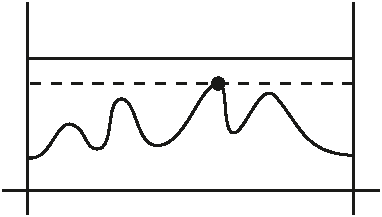
\includegraphics[width=0.4\linewidth]{pictures/26_11_3.pdf}
		\caption{popis}
		\label{fig:26-3}
	\end{figure}
	
	\begin{proof}
		\begin{enumerate}[1)]
			\item Ukážeme, že $\delta_0$ je minimax: sporem $\delta_0$ není minimax, viz obrázek \ref{fig:26-3}. Tím získáme spor s přípustností $\delta_0$.
			\item Jednoznačnost: $\delta_0$ je minimax: sporem. $\exists\delta_1\neq\delta_0$ a přitom $/delta_1$ je minimax.
			\begin{center}
				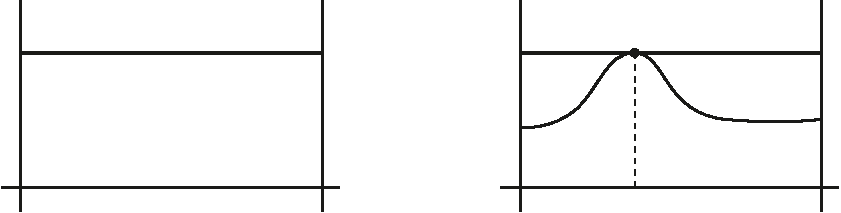
\includegraphics[width=0.7\linewidth]{pictures/26_11_4.pdf}
			\end{center}
		\end{enumerate}
	\end{proof}
\end{theorem}
\subsection{Steinův efekt (paradox) (1955)}
Nechť $\textbf{X}\sim f(\textbf{x},\boldsymbol{\t}),~\boldsymbol{\t}\in\Theta\subset\R^k,~f$ je sféricky symetrické rozdělení okolo $\boldsymbol{\t}$, tzn. $f(\left\|\textbf{x}'-\boldsymbol{\t}\right\|+\left\|\textbf{x}''\right\|)$, kde $\textbf{x}=(\textbf{x}',\textbf{x}''),~\textbf{x}'\in\R^k,~\textbf{x}''\in\R^{n-k}$, např. $\NN_k(\boldsymbol{\t},\I_{k\times k})$,... Volme pro $\boldsymbol{\t}$ váženou kvadratickou $L_2^w(\boldsymbol{\t},\boldsymbol{\delta})=\sum_{j=1}^k w_j(\t_j-\delta_j)^2$. 
	
Označme $\boldsymbol{\delta}^\ast(\textbf{x})=\big(\delta_1^\ast(\textbf{x}),...,\delta_k^\ast(\textbf{x})\big)$ odhad (rozhodovacích funkcí) pro $\boldsymbol{\t}$ klasickou statistickou procedurou. 

Pak $\exists k_0$ tak, že $\forall k\geq k_0$ je $\boldsymbol{\delta}^\ast$ nepřípustným odhadem (rozhodovací funkce) pro $\boldsymbol{\t}$, přestože $\delta_j^\ast$ jsou pro odhad $\t_j$ přípustné $\forall j\in\widehat{k}$.
\begin{dusl}
	Například klasickou rizikovou funkci metodou jednoznačného minimaxu je od $k_0$ beznadějná, protože víme (z nějaké věty), že pokud existuje jednoznačný minimax , pak je přípustný. Stein ale říká, že od $k_0$ klasická statistika nemůže poskytovat přípustný. Tedy stejnoměrně nejlepší strategie od dimenze $k_0$ neexistuje.
\end{dusl}
Co s tím? Místo $\delta_u=\argmin\limits_{\delta\in\mathscr{D}}\RF(\t,\delta),~\forall\t$ hledá $\delta_{pu}=\argmin\limits_{\delta\in\mathscr{D}_0\subset\mathscr{D}}\RF(\t,\delta)$, např. $\mathscr{D}_0$ nestranné odhady (UMVUE). Tím jsme zajistili existenci, ale pro vysokou dimenzi opět dostaneme nepřípustné řešení. Další možností je použít $\mathscr{D}_0'$ jako \textbf{ekvivariantní} odhady. Ty pak vedou na ...něco.

Řešení se pak nabízí v podobě Bayese (začlenění apriorní informace $\pi$).

\begin{description}
	\item[1955 Steinův efekt:] Mějme $X\sim \NN_k(\boldsymbol{\t},\mathbb{I}_{k\times k})$ a nechť $\delta_0(\textbf{x}=\textbf{x})$ je ML, minimaxní a víme, že $\RF(\t,\delta_0)=konst$. Do roku 1955 se myslelo, že $\delta_0$ je jednoznačný minimax $\forall k$. Dle věty o jednoznačnosti minimaxu by bylo $\delta_0$  přípustné $\forall k$. Stein však roku 1955 ukázal, že $\delta_0$ je jednoznačný minimax přípustný pro $k=\hat{2}$ a že pro $(\forall k\geq3)(\exists\delta')(\delta'\ll\delta_0)$.
	  \begin{figure}[h]
		\centering
		\begin{asy}
		unitsize(0.65cm);
		arrowbar myarrow=Arrow;
		void xtick(real x){draw((x,-.1) -- (x,.1));}
		
		void ytick(real y){draw((-.1,y) -- (.1,y));}
		
		path s = ((0,.5) .. (1.5,1.2) .. (3,2) .. (4.5,1.2) .. (6,.5) .. (7,.4));
		draw(s);
		draw((-.1,0) -- (7.1,0));
		draw((0,-.1) -- (0,3));
		draw((6,-.1) -- (6,3));
		dot((3,2));
		draw((0,2)--(7,2));
		ytick(2);
		label("$\mathrm{R}(\theta,\delta_0)$",(3,2.5));
		label("$\left\|\theta\right\|$",(3,-0.5));
		\end{asy}
		\caption{Popis.}\label{pic2}
	\end{figure}
	\item[1961 James-Steinův (shrinkable):]$$ \delta^\mathrm{JS}(\textbf{x})=\underbrace{\Big(1-\frac{k-2}{\left\|\textbf{x}\right\|}\Big)}_{\to-\infty\text{ při }\left\|\textbf{x}\right\|\to0_+}\textbf{x} $$
	\item[1970 Baranchick:] $$ \delta_c^+(\textbf{x})=\Big(1-\frac{c}{\left\|\textbf{x}\right\|^2}\Big)^+\textbf{x}=\begin{cases}
	\big(1-\frac{c}{\left\|\textbf{x}\right\|^2}\big)\textbf{x} & \text{pokud }c<\abs{\textbf{x}}^2 \\0 & \text{jinak,}
	\end{cases} $$
	kde $c\in[k-2,2(k-2)]$. Pak $\delta_c^+\ll \delta_\mathrm{JS} \ll \delta_0,~\forall k\geq 3$.
	\item[1994 Shao et al.] $\exists \delta_S \ll \delta_c^+$, ale vylepšení už nestojí za tu složitost (tedy Baranchick je kompromis v rámci použitelnosti).
\end{description}
\begin{remark}
   Pro $c=2k-1\notin [k-2,2(k-2)]$, $\RF(\t,\delta_{2k-1}^+)$.
   \begin{figure}[h]
   	\centering
   	\begin{asy}
   	unitsize(0.65cm);
   	arrowbar myarrow=Arrow;
   	void xtick(real x){draw((x,-.1) -- (x,.1));}
   	
   	void ytick(real y){draw((-.1,y) -- (.1,y));}
   	
   	path s = ((0,1) .. (2,2.2) .. (4,2.1) .. (6,2));
   	draw(s);
   	draw((-.1,0) -- (7.5,0), arrow=myarrow);
   	draw((0,-.1) -- (0,3), arrow=myarrow);
   	draw((0,2)--(6,2));
   	ytick(2);
   	label("$\mathrm{R}(\theta,\delta_{2k-1}^+)$",(2,0.8));
   	label("$\left\|\theta\right\|$",(8.2,0));
   	label("$\big(\delta_0(\textbf{x})=\textbf{x}\big)~\mathrm{R}(\theta,\delta_0)$",(9,2));
   	label("$k$",(-0.4,2));
   	\end{asy}
   	\caption{Popis.}\label{pic1}
   \end{figure}
\end{remark}
\begin{theorem}[Bergerův jev]
	$\forall k_0\in\N$ (dimenzi $\boldsymbol{\t}$) $\exists L(\boldsymbol{\t},\boldsymbol{\delta})$, že $\boldsymbol{\delta}^\ast(\textbf{x})$ klasickou statistickou procedurou je $\forall k\geq k_0$ nepřípustný.
\end{theorem}

\begin{remark}
	Připomínka: R-B. V. Mějme $L(\t,\delta)$ konvexní v $\delta$ při $\forall\t$, $\pi(\textbf{X})$ je PS, $delta_0$ je libovolná riziková funkce. Pak $\widehat{\delta}(\textbf{t})=\EE{\delta_0(\textbf{X})|\pi(\textbf{X})=\textbf{t}}\ll \delta_0$ a $\E\widehat{\delta}=\E \delta_0$.
\end{remark}
\begin{define}
	Označme $L\big(\t,\delta|\tau(\t)\big)$. Pak $/delta(\textbf{x})$ nazýváme \textbf{nestranná} vzhledem k $L$, pokud $$ \E L\big(\t,\delta|\tau(\t)\big)\leq \E L\big(\t,\delta|\phi(\t))\big),~\forall\phi,\forall\t.$$
\end{define}
$\mathscr{D}_0\subset \mathscr{D}$ jako prostor nestranných rizikových funkcí vzhledem k $L$. Dále
$ \delta_U^0=\argmin_{\delta\in\mathscr{D}_0}\RF(\t,\delta),~\forall\t$ jako UBU$_L$E, pokud existuje. Pak
$$ L=L_2(\t,\boldsymbol{\delta})=(\t-\delta)^2\equal{\text{případně}}\big(\tau(\t)-\delta\big)^2\quad\Rightarrow\quad UMVUE.$$

\begin{theorem}
	Mějme $L$ konvexní v $\delta$, $T(\textbf{X})$ je ÚPS, $\delta_0$ nestranná $L_2$. Pak $\widehat{\delta}_\mathrm{R-B}(\textbf{t})$ je UMVUE (potenciálně nepřípustný).
	
	\begin{figure}[h]
		\centering
		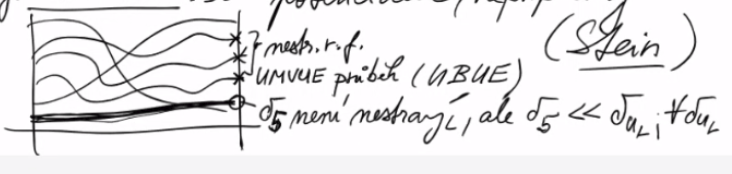
\includegraphics[width=0.6\linewidth]{pictures/3.12-1}
		\caption{popis}
		\label{fig:3}
	\end{figure}
	
\end{theorem}

\section{Equivariantní R. F. (MRE$_q$E)}
\begin{define}
	Mějme grupu $(G,\ast)$, tj. $g_1,g_2\in G~\Rightarrow~ g_1\ast g_2$ a grupu $(R,\ast)$, \[
	\begin{split}
	g\in G,~x\in R&~\Rightarrow g\ast x \\ \textbf{x}\in\R^n&~\Rightarrow~ g\ast \textbf{x}\text{ po složkách }\textbf{x},~\forall g\in G.
	\end{split}
	\]
	Pravděpodobnostní model $X_j=\t\ast \epsilon_j$, kde $\epsilon_j$ značí chyby měření s $\epsilon_j\sim \PP_{0j},~\forall j\in\hat{n}$. $\textbf{X}=(X_j)_{j=1}^n=\t\ast\boldsymbol{\epsilon}$, kde $\boldsymbol{\epsilon}$ je chyba měření s $$\boldsymbol{\epsilon}\stackrel{id}{\sim}\prod_{j=1}^n \PP_{0j}\equal{iid}(\PP_{0j})^n.$$
	Dále platí, že $$ \textbf{X}\sim \PP_\t\in\PP_\ast=\{\PP_\t:\t\in\Theta\subset \R\}~\Rightarrow~ g\in G~\Rightarrow~ g\ast \textbf{X}=g\ast(\t\ast\boldsymbol{\epsilon})=(g\ast\t)\ast\boldsymbol{\epsilon}\sim \PP_{g\ast \t}\in \PP_\ast.$$ 
\end{define}
\begin{theorem}
	Rozhodovací funkce $\delta$ se nazývá ekvivariantní pro $\t$ vzhledem k $(G,\ast)$, pokud $$ \delta(g\ast\textbf{x})=g\ast \delta(\textbf{x}),\quad \forall g\in G,~\forall \textbf{x}\in\chi(\R^n).$$
\end{theorem}
\begin{theorem}
	Ztrátová funkce $L(\t,\delta)$ se nazývá \textbf{invariantní} vzhledem k $(G,\ast)$, pokud $$ L(g\ast\t,g\ast\boldsymbol{\delta})=L(\t,\boldsymbol{\delta}),\quad\forall \t,\forall g,\forall \delta.$$
\end{theorem}
\begin{dusl}
	\[
	\begin{split}
	L(\t,\delta)\equal{\forall g}L(h\ast\t,g\ast \delta)&=\Big| \begin{array}{l}
	\text{volme }g=\tilde{\t}\text{ inverzní prvek v }(G,\ast)\\\text{tzn. }\tilde{\t}\ast\t=I/O\text{ neutrální prvek v }(G,\ast)
	\end{array}
	\Big|=L(\tilde{\t}\ast\t,\tilde{\t}\ast\delta)=\\&=L(I/O,\tilde{\t}\ast\delta)=\rho(\tilde{\t}\ast\delta),\quad\forall\t,\forall\delta.
	\end{split}
	\] 
\end{dusl}
\begin{dusl}
	\[
	\begin{split}
	\RF(\t,\delta)&=\E_\t L\big(\t,\delta(\textbf{X})\big)\equal{inv.~L}\E_\t\rho\big(\tilde{\t}\ast\delta(\textbf{X})\big)=\Big|\begin{array}{l}
	\textbf{x}=\t\ast\boldsymbol{\epsilon}\\\boldsymbol{\epsilon}\sim\PP_0	
	\end{array}
	\Big|=\E_{\PP_0}\rho\big(\tilde{\t}\ast\delta(\t\ast\boldsymbol{\epsilon})\big)\equal{\delta~eqiv.}\\&=\E_{\PP_0}\rho\big(\tilde{\t}\ast\t\ast\delta(\boldsymbol{\epsilon})\big)=\E_{\PP_0}\rho\big(I/O\ast\delta(\boldsymbol{\epsilon})\big)=konst~v~\t,~\forall\t,
	\end{split}
	\]
což nezávisí na $\t$.
\end{dusl}
\begin{define}
	Definujeme $$ \delta^\ast:=\argmin_{\delta\in\mathscr{D}_{Eq}}\RF(\t,\delta),~\forall\t\quad-\text{říkáme }MRE_qE.$$
\end{define}
\begin{example}
	$(G,\ast)=(R,+)$... $g\ast\textbf{x}=(x_1+g,...,x_n+g)=g+\textbf{x}.$Pravděpodobnostní model se na Location family
	\[
\begin{split}
X_j&=\t+\epsilon_j\quad(\text{aditivní chyba})\\
\textbf{x}&=\t+\boldsymbol{\epsilon}\sim\PP_\t\text{ a platí, že }\\
g\ast \textbf{X}&=g+\textbf{X}\sim \PP_{g+\t}.
\end{split}
\]
	$\delta$ je ekvivariantní, pokud $\delta(g+\textbf{x})=g+\delta(\textbf{x})$, např. $\delta(\textbf{x})=\frac{1}{n}\sumjn X_j$ je ekvivariantní rifizová funkce, protože $\delta(g+\textbf{x})=\frac{1}{n}\sumjn (X_j+g)=\frac{1}{n}\sumjn X_j + g=\delta(\textbf{x})+g$. $L$ invariantní znamená, že $L(\t,\delta)=\rho(\tilde{\t}\ast\delta)=\rho(\delta-\t)\equal{\text{např.}}(\delta-\t)^2=L_2$.
\end{example}

Závěr: Existuje procedura pro hledání $MSE_qE$ .. pro $(G,\ast)=(R,+)$ ve tvaru
$$ \delta^\ast(\textbf{x})=\argmin_{\delta\in\mathscr{D}_{Eq}}\frac{\int\rho(\delta-\t)f(\textbf{x}-\t)\d\t}{\int f(\textbf{x}-\t)\d\t}=\delta_B^{\pi=1}(\textbf{x}).$$

\begin{remark}
	Připomínka: $\widehat{\delta_B}=\argmin_\delta r(\pi,\delta)$ nebo $\widehat{\delta_B}(\textbf{x})=\argmin_{\delta(\textbf{x})}\rho(\pi,\delta|\textbf{x})$, kde 
	$$ \rho(\pi,\delta|\textbf{x})=\E^\pi[L|\textbf{x}]=\int L(\t,\delta)\pi(\t|\textbf{x})\d\t=\int L(\t,\delta)\frac{f \pi(\t)}{\int f \pi(\t)\d\t}\d\t.$$
 Zde stačí volit $\pi(\t)=1$ na $\Theta$. Pokud zvolíme konkrétně $L=L_2$, pak $\delta^\ast(\textbf{x})=\frac{\int\t f(\textbf{x}-\t)\d\t}{\int f(\textbf{x}-\t)\d\t}$, což se nazývá \textbf{Pitmanův odhad}.
\end{remark}
\begin{example}
	Mějme $\epsilon_j~iid~\mathrm{Exp}(1)$, $f(\textbf{x}-\boldsymbol{\t})=\e{-\sumjn x_j+n\t}$, pokud $\t< x_{(1)}=\min (x_j)_1^n$. Dále pak
	$$ \delta^\ast(\textbf{x})\equal{L_2}...=x_{(1)}-\frac{1}{n},$$ což je Pitmanův odhad pro $\mathrm{Exp}(1)$, tedy $MRE_qE$.
\end{example}

%########################## LESSON 10.12
\begin{theorem}\label{veta1}
	Mějme $X\sim \fex(x|\t),~\pi(\t)\sim \t,L_2$ (ÚBM). Pokud $0<\E(\t^2|\textbf{x})<+\infty$, pak $\delta^\pi(\textbf{x})=\E^\pi(\t|\textbf{x})$, kde $$\pi(\t|\textbf{x})=\frac{f(x|\t)\pi(\t)}{\int_\Theta f(x|\t)\pi(\t)\d\t}.$$
\end{theorem}

\begin{theorem}
	Mějme $\fex,~\pi(\t),~L_2^w(\t,\delta)=w(\t)(\t-\delta)^2$. Pokud $0<\EE{\t^2w(\t)}<+\infty$, pak $$\delta^\pi(\textbf{x})=\frac{\E^\pi{\t w(\t)|\textbf{x}}}{\EE{w(\t)|\textbf{x}}}$$
	a $r(\pi)=c\E^{m_w}[\D^{\pi_w}(\t|\textbf{x})]$, kde $m_w^{(*)}$ a $\pi_w(\t|\textbf{x})$ jsou marginální rozdělení $\textbf{X}$ a $\t|\textbf{x}$ příslušné $\pi_w(\t)=\frac{\pi(\t)w(\t)}{c}$, $c=\int\pi w\d\t$.
	\begin{proof}
		\[
		\begin{split}
		r_w(\pi,\delta)&\stackrel{L_2^w}{\equiv}\E^\pi\big[\E^f[L_2^w(\t,\delta(\textbf{X}))]\big]=\int_\Theta\Big(\int_{\chi(\R^n)} w(\t)\big(\t-\delta(\textbf{x})\big)^2 f(\textbf{x}|\t)\d\textbf{x}\Big)\pi(\t)\d\t=\\
		&= \int_\Theta \E\big[L_2\big(\t,\delta(\textbf{X})\big)\big]\underbrace{ \pi(\t)w(\t)}_{\propto \pi_w(\t)c}\d\t = c\E^{\pi_w}\underbrace{\E^f (L_2)}_{\RF(\t,\delta)}=cr_2(\pi_w,\delta).
		\end{split}
		\]
		Ukázali jsme tedy, že  
		$$\delta^\pi=\argmin_\delta r_w(\pi,\delta)=\argmin_\delta r_2(\pi_w,\delta)\stackrel{\ref{veta1}}{=}\E^{\pi_w}(\t|\textbf{x}),$$
		kde $\pi_w(\t|\textbf{x})$ příslušné $\pi_w(\t)$. Z toho se dá vyjádřit, že $r(\pi)\stackrel{\ref{veta1}}{=}\E^{m_w}\D^{\pi_w}(\t|\textbf{x})$.
	\end{proof}
\end{theorem}
\begin{remark}\begin{itemize}
		\item $w(\t)$ výrazně ovlivňuje Bayesovské řešení.
		\item $\delta^\pi$ je jednoznačný, potom je přípustný. $\RF(\t,\delta)$ je spojitá v $\t$ a $\pi>0\Rightarrow\delta^\pi$ je přípustná, přípustná $\delta^\pi$ není ovlivněna $w(\t)$ v $L_2^w$ (robustnost $/delta^\pi$).
	\end{itemize}
\end{remark}

\begin{theorem}
	Mějme $\big\{ f(x|\bt):\bt\in\Theta\subset\R^k \big\},~\bt\sim\pi(\bt),~L=L_2^Q(\bt,\bdelta)=(\bt-\bdelta)^T\Q(\bt-\bdelta)$, kde $\Q$ je PD matice o rozměru $k\times k $ a $\Q$ nezávisí na $\bt$. Nechť $\Cov(\bt|\textbf{x})=\D(\bt|\textbf{x})$ je konečná (ideálně regulární), nenulová. Pak $\bdelta^\pi(\textbf{x})=\E^\pi(\bt|\textbf{x})$. 
	\begin{proof}
		Obdodně jako v $\R^1$.
	\end{proof}
\end{theorem}
\begin{remark}
	\begin{enumerate}[a)]
		\item $\delta^\pi$ nezávisí na tvaru $\Q$, tzn. volíme $\Q=\I$ a nemusíme užívat $L_2^\Q=\sum_i\sum_j q_{ij}(\t_i-\delta_i)(\t_j-\delta_j)$.
		\item $L_2^{\Q,\textbf{w}}(\bt,\bdelta)=\sum_1^k w_i(\t_i-\delta_i)^2$. Neplatí V3! 
	\end{enumerate}
\end{remark}
Další volby L?
$L_2$ není robustní (1964 Huber, Hampel, Ronchetti). 

$$ L_p,~p\in(1,2)=(\t-\delta)^p.$$

$$\delta^\pi=\argmin_\delta \underbrace{r(\pi,\delta)}_{\E^\pi\E^f L}\stackrel{\forall\textbf{x}}{=}\argmin_{\delta(\textbf{x})}\underbrace{\rho(\pi,\delta|\textbf{x})}_{\E^\pi(L|\textbf{x})=\int L\big(\t,\delta(\textbf{x})\big)\pi(\t|\textbf{x})\d\t}.$$


\begin{theorem}\begin{enumerate}[a:]
		\item $f(x,\t),~\pi(\t),~L=L_1(\t,\delta)=|\t-\delta|$. Nechť $0<\EE{|\t|\big|\textbf{x}}<+\infty$, pak $\delta^\pi(\textbf{x})=\pi_{1/2}(\t|\textbf{x})$ medián aposteriorního rozdělení.
		\item $f,~\pi,~L=L_{k_1,k_2}(\t,\delta)=\begin{cases}
		k_1(\delta-\t)&\delta\geq \t \\ k_2(\t-\delta)& \delta<\t.
		\end{cases}$ (multilineární loss). Nechť $0<\E\big(|\t|\big|\textbf{x}\big)<+\infty$. Pak $\delta^\pi(\textbf{x})=\pi_{\frac{k_2}{k_1+k_2}}(\t|\textbf{x})$, $\frac{k_2}{k_1+k_2}$ je kvantil aposteriorního rozdělení.
		\begin{figure}[h]
			\centering
			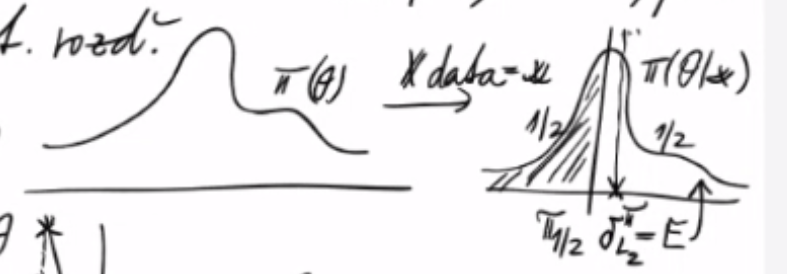
\includegraphics[width=0.7\linewidth]{pictures/10.12}
			\caption{popis}
			\label{fig:10}
		\end{figure}
		
		\begin{proof}
			\[
			\begin{split}
			\rho(\pi,&\delta|\textbf{x})=\big[L_{k_1,k_2}(\t,\delta\big| \textbf{x})\big]=k_1\int_{-\infty}^\delta (\delta-\t)\pi(\t|\textbf{x})\d\t+k_2\int_\delta^{+\infty}(\t-\delta)\pi(\t|\textbf{x})\d\t\stackrel{P.P.}{=}\\&=k_1\Big(\big[(\delta-\t)\FF_\pi(\t|\textbf{x})\big]_{-\infty}^\delta+\int_{-\infty}^\delta \FF_\pi(\t|\textbf{x})\d\t\Big)+k_2(DCv.)\Big)=\\&=k_1\Big( 0-\underbrace{\delta\FF_\pi(-\infty|\textbf{x})}_{0}+\underbrace{\lim\limits_{\t\to+\infty}\t\FF_\pi(\t|\textbf{x})}_{0\text{, protože }\int_\Theta |\t|\pi(\t|\textbf{x})<\infty}+\int_{-\infty}^\delta \FF_\pi(\t|\textbf{x})\d\t \Big)+k_2\Big( []_\delta^{+\infty}-\int_\delta^{+\infty}\FF_\pi \d\t \Big)=\\&=k_1\int_{-\infty}^\delta \FF_\pi(\t|\textbf{x})\d\t+k_2\int_\delta^{+\infty}\big(1-\FF_\pi(\t|\textbf{x})\big)\d\t.
			\end{split}
			\]
			\[
			\begin{split}
			\rho_\delta'&=k_1\cdot 1\cdot\FF_\pi(\delta|\textbf{x})+k_2\cdot(-1)\big(1-\FF_\pi(\delta|\textbf{x})\big)=0,\\\delta(\textbf{x})&=\pi_{\frac{k_2}{k_1+k_2}}(\t|\textbf{x}) \Leftarrow \FF_\pi(\delta|\textbf{x})=\frac{k_2}{k_1+k_2}\in(0,1)
			\end{split}
			\]
		\end{proof} 
	\end{enumerate}
	
\end{theorem}
\begin{theorem}
	Mějme $f,~\pi,~L=L_{\{0,1\}}(\t,\delta)\equal{ozn}L_{0,1}(\t,\delta)=\begin{cases}
	0&|\t-\delta|\leq c,\\1& |\t-\delta|>c.
	\end{cases}$. Pak $\delta^\pi(\textbf{x})$ je středem intervalu $I_{2c}$ délky $2c$, který maximalizuje $\PP^\pi(\t\in I_{2c}|\textbf{x})$.
	\begin{proof}
		Přenecháno čtenáři.
	\end{proof}
\begin{figure}[h]
	\centering
	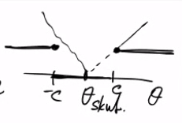
\includegraphics[width=0.7\linewidth]{pictures/10.12-2}
	\caption{popis}
	\label{fig:105}
\end{figure}
\end{theorem}

\begin{define}
	$c\to 0+$ definujeme \textbf{maximum aposteriori rohodovací funkce} vztahem $\delta_\mathrm{MAP}(\textbf{x})=\argmax_\t \pi(\t|\textbf{x})$. Pak $$\delta_\mathrm{MAP}(\textbf{x})=\argmax_\t f(\textbf{x}|\t)\pi(\t).$$
\end{define}


